\documentclass[10pt,landscape]{article}
\usepackage{multicol}
\usepackage{calc}
\usepackage{ifthen}
\usepackage[landscape]{geometry}
\usepackage{graphicx}
\usepackage{amsmath, amssymb, amsthm}
\usepackage{latexsym, marvosym}
\usepackage{pifont}
\usepackage{lscape}
\usepackage{graphicx}
\usepackage{array}
\usepackage{booktabs}
\usepackage[bottom]{footmisc}
\usepackage{tikz}
\usetikzlibrary{shapes}
\usepackage{pdfpages}
\usepackage{wrapfig}
\usepackage{enumitem}
\setlist[description]{leftmargin=0pt}
\usepackage{xfrac}
\usepackage[pdftex,
            pdfauthor={William Chen},
            pdftitle={Probability Cheatsheet},
            pdfsubject={A cheatsheet pdf and reference guide originally made for Stat 110, Harvard's Introduction to Probability course. Formulas and equations for your statistics class.},
            pdfkeywords={probability} {statistics} {cheatsheet} {pdf} {cheat} {sheet} {formulas} {equations}
            ]{hyperref}
\usepackage[
            open,
            openlevel=2
            ]{bookmark}
\usepackage{relsize}
\usepackage{rotating}

 \newcommand\independent{\protect\mathpalette{\protect\independenT}{\perp}}
    \def\independenT#1#2{\mathrel{\setbox0\hbox{$#1#2$}%
    \copy0\kern-\wd0\mkern4mu\box0}} 
            
\newcommand{\noin}{\noindent}    
\newcommand{\logit}{\textrm{logit}} 
\newcommand{\var}{\textrm{Var}}
\newcommand{\cov}{\textrm{Cov}} 
\newcommand{\corr}{\textrm{Corr}} 
\newcommand{\N}{\mathcal{N}}
\newcommand{\Bern}{\textrm{Bern}}
\newcommand{\Bin}{\textrm{Bin}}
\newcommand{\Beta}{\textrm{Beta}}
\newcommand{\Gam}{\textrm{Gamma}}
\newcommand{\Expo}{\textrm{Expo}}
\newcommand{\Pois}{\textrm{Pois}}
\newcommand{\Unif}{\textrm{Unif}}
\newcommand{\Geom}{\textrm{Geom}}
\newcommand{\NBin}{\textrm{NBin}}
\newcommand{\Hypergeometric}{\textrm{HGeom}}
\newcommand{\HGeom}{\textrm{HGeom}}
\newcommand{\Mult}{\textrm{Mult}}

\geometry{top=.4in,left=.2in,right=.2in,bottom=.4in}

\pagestyle{empty}
\makeatletter
\renewcommand{\section}{\@startsection{section}{1}{0mm}%
                                {-1ex plus -.5ex minus -.2ex}%
                                {0.5ex plus .2ex}%x
                                {\normalfont\large\bfseries}}
\renewcommand{\subsection}{\@startsection{subsection}{2}{0mm}%
                                {-1explus -.5ex minus -.2ex}%
                                {0.5ex plus .2ex}%
                                {\normalfont\normalsize\bfseries}}
\renewcommand{\subsubsection}{\@startsection{subsubsection}{3}{0mm}%
                                {-1ex plus -.5ex minus -.2ex}%
                                {1ex plus .2ex}%
                                {\normalfont\small\bfseries}}
\makeatother

\setcounter{secnumdepth}{0}

\setlength{\parindent}{0pt}
\setlength{\parskip}{0pt plus 0.5ex}

% -----------------------------------------------------------------------

\usepackage{titlesec}

\titleformat{\section}
{\color{blue}\normalfont\large\bfseries}
{\color{blue}\thesection}{1em}{}
\titleformat{\subsection}
{\color{cyan}\normalfont\normalsize\bfseries}
{\color{cyan}\thesection}{1em}{}
% Comment out the above 5 lines for black and white

\begin{document}

\raggedright
\footnotesize
\begin{multicols*}{3}

% multicol parameters
% These lengths are set only within the two main columns
%\setlength{\columnseprule}{0.25pt}
\setlength{\premulticols}{1pt}
\setlength{\postmulticols}{1pt}
\setlength{\multicolsep}{1pt}
\setlength{\columnsep}{2pt}

%%%%%%%%%%%%%%%%%%%%%%%%%%%%%%%%%%%%
%%% TITLE
%%%%%%%%%%%%%%%%%%%%%%%%%%%%%%%%%%%%

\begin{center}
    {\color{blue} \Large{\textbf{Probability Cheatsheet v2.0}}} \\
   % {\Large{\textbf{Probability Cheatsheet}}} \\
    % comment out line with \color{blue} and uncomment above line for b&w
\end{center}

%%%%%%%%%%%%%%%%%%%%%%%%%%%%%%%%%%%%
%%% ATTRIBUTIONS
%%%%%%%%%%%%%%%%%%%%%%%%%%%%%%%%%%%%

\scriptsize

Compiled by William Chen (\url{http://wzchen.com}) and Joe Blitzstein, with contributions from Sebastian Chiu, Yuan Jiang, Yuqi Hou, and Jessy Hwang. Material based on Joe Blitzstein's (\texttt{\href{http://twitter.com/stat110}{@stat110}}) lectures (\url{http://stat110.net}) and Blitzstein/Hwang's Introduction to Probability textbook (\url{http://bit.ly/introprobability}). Licensed under \texttt{\href{http://creativecommons.org/licenses/by-nc-sa/4.0/}{CC BY-NC-SA 4.0}}. Please share comments, suggestions, and errors at \url{http://github.com/wzchen/probability_cheatsheet}.

\begin{center}
    Last Updated \today
\end{center}

% Cheatsheet format from
% http://www.stdout.org/$\sim$winston/latex/

%%%%%%%%%%%%%%%%%%%%%%%%%%%%%%%%%%%%
%%% BEGIN CHEATSHEET
%%%%%%%%%%%%%%%%%%%%%%%%%%%%%%%%%%%%


\section{Counting}\smallskip \hrule height 2pt \smallskip

% \subsection{Set Theory}

% \begin{description}
%     \item[Sets and Subsets] - A set is a collection of distinct objects. $A$ is a subset of $B$ if every element of $A$ is also included in $B$.
%     \item[Empty Set] - The empty set, denoted $\emptyset$, is the set that contains nothing.
%     \item[Set Notation] - Note that ${\bf {\bf A}} \cup {\bf B}$, ${\bf A} \cap {\bf B}$, and ${\bf A^c}$ are all sets too.
%     \begin{description}
%         \item[Union] - ${\bf A} \cup {\bf B}$ (read \emph{{\bf A} union {\bf B}}) means ${\bf A}\ or\ {\bf B}$
%         \item[Intersection] - ${\bf A} \cap {\bf B}$ (read \emph{{\bf A} intersect {\bf B}}) means ${\bf A}\ and \ {\bf B}$
%         \item[Complement] - ${\bf A^c}$ (read \emph{{\bf A} complement}) occurs whenever ${\bf A}$ does not occur
%     \end{description}
%     \item[Disjoint Sets] - Two sets are disjoint if their intersection is the empty set (e.g. they don't overlap).
%     \item[Partition] - A set of subsets ${\bf A}_1, {\bf A}_2, {\bf A}_3, ... {\bf A}_n$ partition a space if they are disjoint and cover all possible outcomes (e.g. their union is the entire set). A simple case of a partitioning set of subsets is ${\bf A}, {\bf A^c}$
%         \item[Principle of Inclusion-Exclusion] - Helps you find the probabilities of unions of events. 
%         \[ P ({\bf A} \cup {\bf B}) = P({\bf A}) + P({\bf B}) - P({\bf A} \cap {\bf B}) \]
%         \[P(\textnormal{Union of many events}) = \textnormal{Singles} - \textnormal{Doubles} + \textnormal{Triples} - \textnormal{Quadruples} \dots\]


% \end{description}
    \subsection{Multiplication Rule} 
    \begin{minipage}{\linewidth}
            \centering
            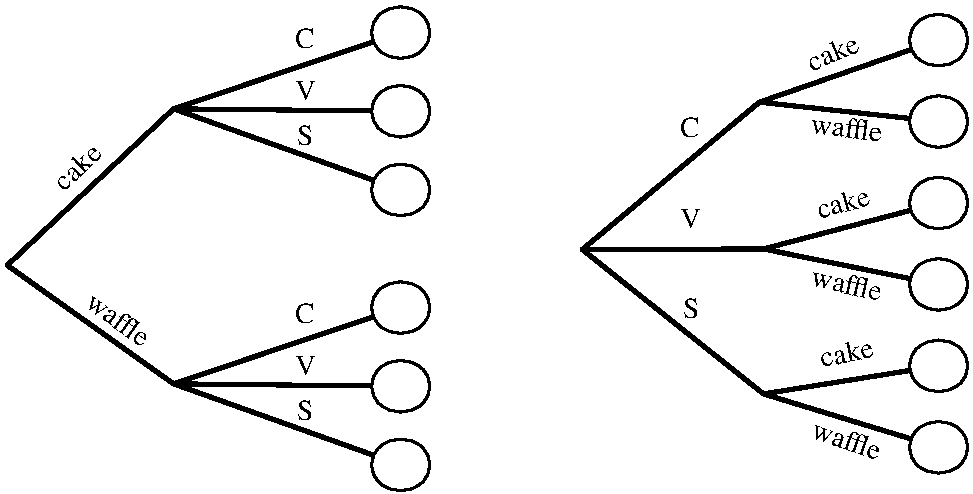
\includegraphics[width=2in]{figures/icecream.pdf}
        \end{minipage}
        
 Let's say we have a compound experiment (an experiment with multiple components). If the 1st component has $n_1$ possible outcomes, the 2nd component has $n_2$ possible outcomes, \dots, and the $r$th component has $n_r$ possible outcomes, then overall there are $n_1n_2 \dots n_r$ possibilities for the whole experiment.
 
\subsection{Sampling Table}
   \begin{minipage}{\linewidth}
            \centering
             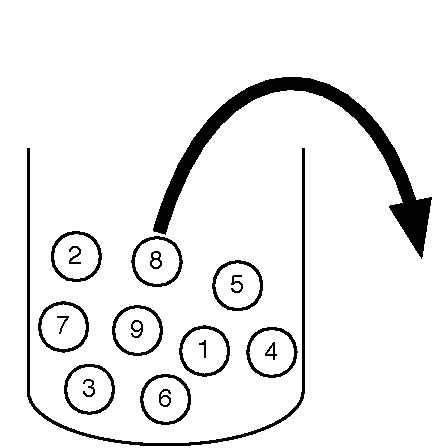
\includegraphics[width=1.2in]{figures/jar.pdf}
        \end{minipage}
      %  \begin{center}
    The sampling table gives the number of possible samples of size $k$ out of a population of size $n$, under various assumptions about how the sample is collected. 
        %\begin{table}[H]
        \begin{center}
                \setlength{\extrarowheight}{7pt}
            \begin{tabular}{r|cc}
                 & \textbf{Order Matters} & \textbf{Not Matter} \\ \hline
                \textbf{With Replacement} & $\displaystyle n^k$ & $\displaystyle{n+k-1 \choose k}$ \\
                \textbf{Without Replacement} & $\displaystyle\frac{n!}{(n - k)!}$ & $\displaystyle{n \choose k}$
            \end{tabular}
        \end{center}
        %\end{table}
    % \item[Experiments/Outcomes] - An experiment generates an outcome from a pre-determined list. For example, a dice roll generates outcomes in the set $\{1, 2, 3, 4, 5, 6\}$
    % \item[Sample Space] - The sample space, denoted $\Omega$, is the set of possible outcomes. Note that the probability of this event is 1, since something in the sample space will always occur.
    % \item[Event] - An event is a subset of the sample space, or a collection of possible outcomes of an experiment. We say that the event has occurred if any of the outcomes in the event have happened.
    \subsection{Naive Definition of Probability}  {If all outcomes are equally likely}, the probability of an event $A$ happening is:
        \[P_{\textrm{naive}}(A) = \frac{\textnormal{number of outcomes favorable to $A$}}{\textnormal{number of outcomes}}\]

\section{Thinking Conditionally} \smallskip \hrule height 2pt \smallskip

% \subsection{Set Theory and Statistics}
% %To understand probability it helps to understand basic set theory. An \emph{event} is a set in that it is a collection of possible outcomes of an experiment (or a subset of the sample space). With set theory we can talk about things like unions, intersections, or complements of events.

% \begin{description}
%     \item[Experiments/Outcomes] - An experiment generates an outcome from a pre-determined list. For example, a dice roll generates outcomes in the set $\{1, 2, 3, 4, 5, 6\}$
%     \item[Sample Space] - The sample space, denoted $\Omega$, is the set of possible outcomes. Note that the probability of this event is 1, since something in the sample space will always occur.
%     \item[Event] - An event is a subset of the sample space, or a collection of possible outcomes of an experiment. We say that the event has occurred if any of the outcomes in the event have happened.
% \end{description}

%\subsection{Disjointness Versus Independence}
\subsection{Independence}

    \begin{description}
        % \item[Disjoint Events] - ${\bf A}$ and ${\bf B}$ are disjoint when they cannot happen simultaneously, or
        %   \begin{align*}
        %     P({\bf A} \cap {\bf B}) &= 0\\
        %     {\bf A} \cap {\bf B} &= \emptyset
        %   \end{align*}
        \item[Independent Events] $A$ and $B$ are independent if knowing whether $A$ occurred gives no information about whether $B$ occurred. More formally, $A$ and $B$ (which have nonzero probability) are independent if and only if one of the following equivalent statements holds: 
           \begin{align*} 
            P({A}\cap { B}) &= P({A})P({B}) \\
            P({ A}|{ B}) &= P({A})\\
            P(B|A) &= P(B)
           \end{align*}
        \item[Conditional Independence]  ${A}$ and ${B}$ are conditionally independent given ${C}$ if $P({A}\cap {B}|{C}) = P({A}|{C})P({B}|{C})$. Conditional independence does not imply independence, and independence does not imply conditional independence.
    \end{description}
    
\subsection{Unions, Intersections, and Complements}

    \begin{description}

        \item[De Morgan's Laws] A useful identity that can make calculating probabilities of unions easier by relating them to intersections, and vice versa. Analogous results hold with more than two sets.
           \begin{align*} 
        ({A} \cup { B})^c = {A^c} \cap { B^c} \\
        ({A} \cap {B})^c = { A^c} \cup { B^c}
           \end{align*} 
                  
        % \item[Complements] - The following are true.
        %    \begin{align*} 
        %      {\bf A} \cup {\bf A}^c &= \Omega \\
        %      {\bf A} \cap {\bf A}^c &= \emptyset\\
        %      P({\bf A}) &= 1 -  P({\bf A}^c)
        %    \end{align*} 

    \end{description}

\subsection{Joint, Marginal, and Conditional}

    \begin{description}
        \item[Joint Probability] $P({A} \cap {B}) $ or $P({ A}, {B})$ -- Probability of ${ A}$ and ${B}$.
        \item[Marginal (Unconditional) Probability] $P({A})$ -- Probability of ${A}$.
        \item[Conditional Probability]  $P({A}|{B}) = P(A,B)/P(B)$ -- Probability of ${A}$, given that ${B}$ occurred.
        \item[Conditional Probability \emph{is} Probability]  $P({A}|{ B})$ is a probability function for any fixed $B$. Any theorem that holds for probability also holds for conditional probability.
    %     \item[Bayes' Rule] - Bayes' Rule unites marginal, joint, and conditional probabilities. We use this as the definition of conditional probability.
    % \[P({\bf A}|{\bf B}) = \frac{P({\bf A} \cap {\bf B})}{P({\bf B})} = \frac{P({\bf B}|{\bf A})P({\bf A})}{P({\bf B})}\]
    \end{description}

\subsection{Probability of an Intersection or Union}
\textbf{Intersections via Conditioning}
\begin{align*} 
    P(A,B) &= P(A)P(B|A) \\
   P(A,B,C) &= P(A)P(B|A)P(C|A,B) 
   \end{align*}
   \textbf{Unions via Inclusion-Exclusion}
   \begin{align*} 
    P(A \cup B) &= P(A) + P(B) - P(A \cap B) \\
  P(A \cup B \cup C) &= P(A) + P(B) + P(C) \\
&\quad - P(A \cap B) - P(A \cap C) - P(B \cap C) \\
&\quad + P(A \cap B \cap C).
   \end{align*}


\subsection{Simpson's Paradox}
\begin{minipage}{\linewidth}
            \centering
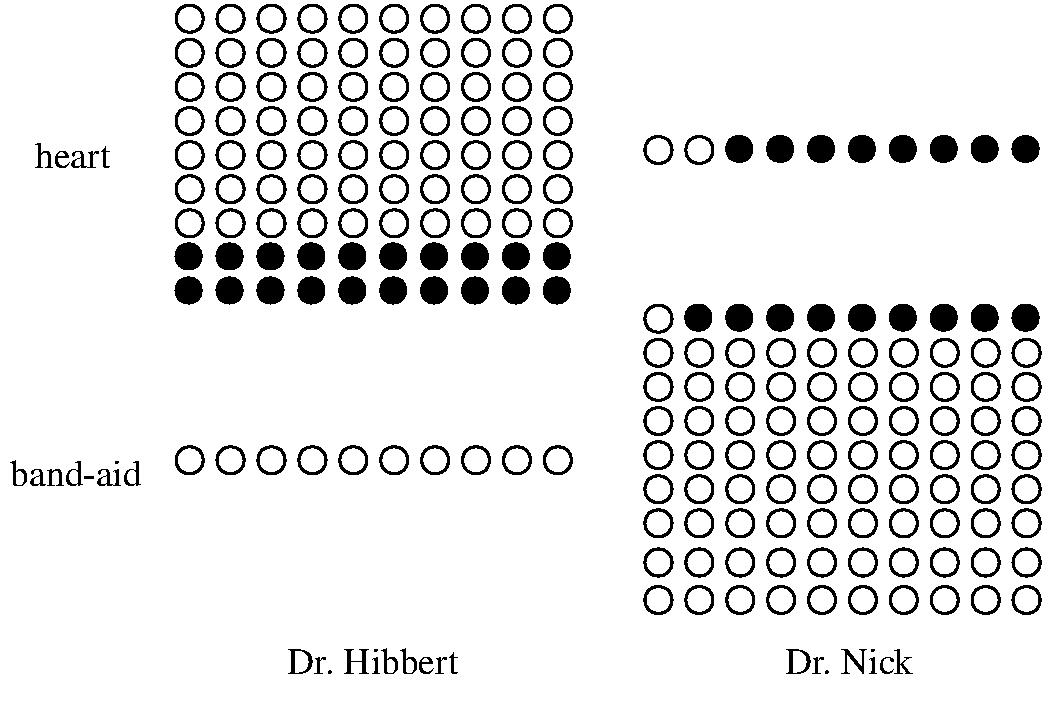
\includegraphics[width=2in]{figures/SimpsonsParadox.pdf}
        \end{minipage}
 It is possible to have
\[P(A\mid B,C) < P(A\mid B^c, C) \textnormal{ and } P(A\mid B, C^c) < P(A \mid B^c, C^c)\]
\[ \textnormal{yet also } P(A\mid B) > P(A \mid B^c).\]
    
\subsection{Law of Total Probability (LOTP)}
Let ${ B}_1, { B}_2, { B}_3, ... { B}_n$ be a \emph{partition} of the sample space (i.e., they are disjoint and their union is the entire sample space).
\begin{align*} 
    P({ A}) &= P({ A} | { B}_1)P({ B}_1) + P({ A} | { B}_2)P({ B}_2) + \dots + P({ A} | { B}_n)P({ B}_n)\\
    P({ A}) &= P({ A} \cap { B}_1)+ P({ A} \cap { B}_2)+ \dots + P({ A} \cap { B}_n)
    \end{align*} 
    For \textbf{LOTP with extra conditioning}, just add in another event $C$!
    \begin{align*} 
    P({ A}| { C}) &= P({ A} | { B}_1, { C})P({ B}_1 | { C}) + \dots +  P({ A} | { B}_n, { C})P({ B}_n | { C})\\
    P({ A}| { C}) &= P({ A} \cap { B}_1 | { C})+ P({ A} \cap { B}_2 | { C})+ \dots +  P({ A} \cap { B}_n | { C})
\end{align*} 

Special case of LOTP with ${ B}$ and ${ B^c}$ as partition:
   \begin{align*} 
P({ A}) &= P({ A} | { B})P({ B}) + P({ A} | { B^c})P({ B^c}) \\
P({ A}) &= P({ A} \cap { B})+ P({ A} \cap { B^c}) \\
   \end{align*} 
   
\subsection{Bayes' Rule}

\textbf{Bayes' Rule, and with extra conditioning (just add in $C$!)}
         \[P({ A}|{ B})  = \frac{P({ B}|{ A})P({ A})}{P({ B})}\]
         \[P({ A}|{ B}, { C}) = \frac{P({ B}|{ A}, { C})P({ A} | { C})}{P({ B} | { C})}\]
         We can also write
         $$P(A|B,C) = \frac{P(A,B,C)}{P(B,C)} = \frac{P(B,C|A)P(A)}{P(B,C)}$$
\textbf{Odds Form of Bayes' Rule}
\[\frac{P({ A}| { B})}{P({ A^c}| { B})} = \frac{P({ B}|{ A})}{P({ B}| { A^c})}\frac{P({ A})}{P({ A^c})}\]
The \emph{posterior odds} of $A$ are the \emph{likelihood ratio} times the \emph{prior odds}. 

\section{Random Variables and their Distributions}\smallskip \hrule height 2pt \smallskip

% \subsection{Conditioning is the Soul of Statistics}

% Law of Total Probability with ${\bf B}$ and ${\bf B^c}$ (special case of a partitioning set), and with Extra Conditioning (just add C!)
%    \begin{align*} 
% P({\bf A}) &= P({\bf A} | {\bf B})P({\bf B}) + P({\bf A} | {\bf B^c})P({\bf B^c}) \\
% P({\bf A}) &= P({\bf A} \cap {\bf B})+ P({\bf A} \cap {\bf B^c}) \\
% P({\bf A} | {\bf C}) &= P({\bf A} | {\bf B}, {\bf C})P({\bf B} | {\bf C}) + P({\bf A} | {\bf B^c}, {\bf C})P({\bf B^c} | {\bf C}) \\
% P({\bf A} | {\bf C}) &= P({\bf A} \cap {\bf B} | {\bf C})+ P({\bf A} \cap {\bf B^c} | {\bf C})
%    \end{align*} 
   
% Law of Total Probability with a partitioning ${\bf B}_0, {\bf B}_1, {\bf B}_2, {\bf B}_3, \dots, {\bf B}_n$, and applied to random variables ${\bf X}$, ${\bf Y}$.
% \begin{align*} 
% P({\bf A}) &= \sum_{i=0}^n P({\bf A} | {\bf B}_i)P({\bf B}_i) \\
% P({\bf Y}=y) &= \sum_{k}P({\bf Y}=y|{\bf X}=k)P({\bf X}=k)
%    \end{align*} 
% Bayes' Rule, and with Extra Conditioning (just add C!)
%     \begin{align*}
%          P({\bf A}|{\bf B}) &= \frac{P({\bf A} \cap {\bf B})}{P({\bf B})} = \frac{P({\bf B}|{\bf A})P({\bf A})}{P({\bf B})} \\
%          P({\bf A}|{\bf B}, {\bf C}) &= \frac{P({\bf A} \cap {\bf B} | {\bf C})}{P({\bf B} | {\bf C})} = \frac{P({\bf B}|{\bf A}, {\bf C})P({\bf A} | {\bf C})}{P({\bf B} | {\bf C})} 
%     \end{align*}
    
\subsection{PMF, CDF, and Independence}
\begin{description}

\item[Probability Mass Function (PMF)] 
Gives the probability that a \emph{discrete} random variable takes on the value $x$.
\[ p_X(x) = P(X=x) \]
\begin{minipage}{\linewidth}
            \centering
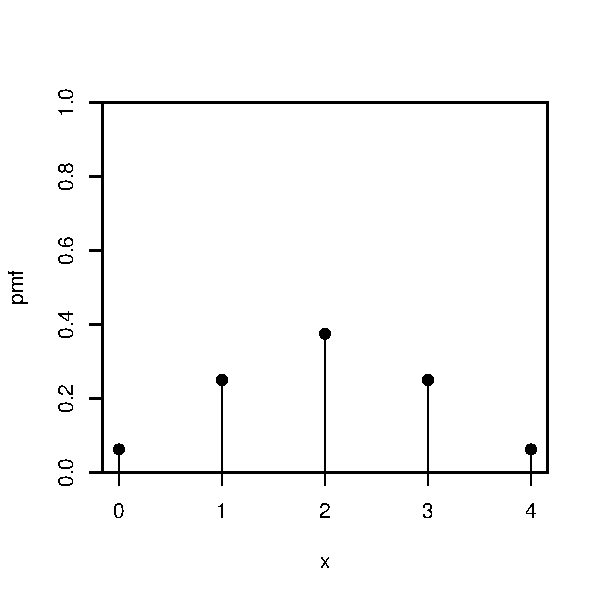
\includegraphics[width=2in]{figures/Binpmf.pdf}
        \end{minipage}
The PMF satisfies
\[p_X(x) \geq 0 \textrm{ and } \sum_x p_X(x) = 1 \]


\item[Cumulative Distribution Function (CDF)] 
Gives the probability that a random variable is less than or equal to $x$.
\[F_X(x) = P(X \leq x)\]
\begin{minipage}{\linewidth}
            \centering
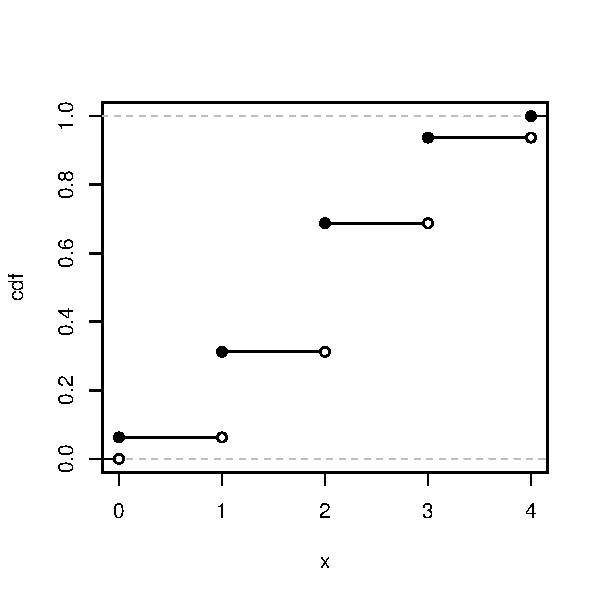
\includegraphics[width=2in]{figures/Bincdf.pdf}
        \end{minipage}

The CDF is an increasing, right-continuous function with
\[F_X(x) \to 0 \textrm{ as $x \to -\infty$ and } F_X(x) \to 1 \textrm{ as $x \to \infty$} \]
\item[Independence] Intuitively, two random variables are independent if knowing the value of one gives  no information about the other. Discrete r.v.s $X$ and $Y$ are independent if for \emph{all} values of $x$ and $y$  \begin{center}
$P(X=x, Y=y) = P(X = x)P(Y = y)$
\end{center}

\end{description}

\section{Expected Value and Indicators}\smallskip \hrule height 2pt \smallskip


\subsection{Expected Value and Linearity}
\begin{description}
\item[Expected Value] (a.k.a.~\emph{mean}, \emph{expectation}, or \emph{average}) is a weighted average of the possible outcomes of our random variable. Mathematically, if $x_1, x_2, x_3, \dots$ are all of the distinct possible values that $X$ can take, the expected value of $X$ is
\begin{center}
$E(X) = \sum\limits_{i}x_iP(X=x_i)$
\end{center}

\begin{minipage}{\linewidth}
            \centering
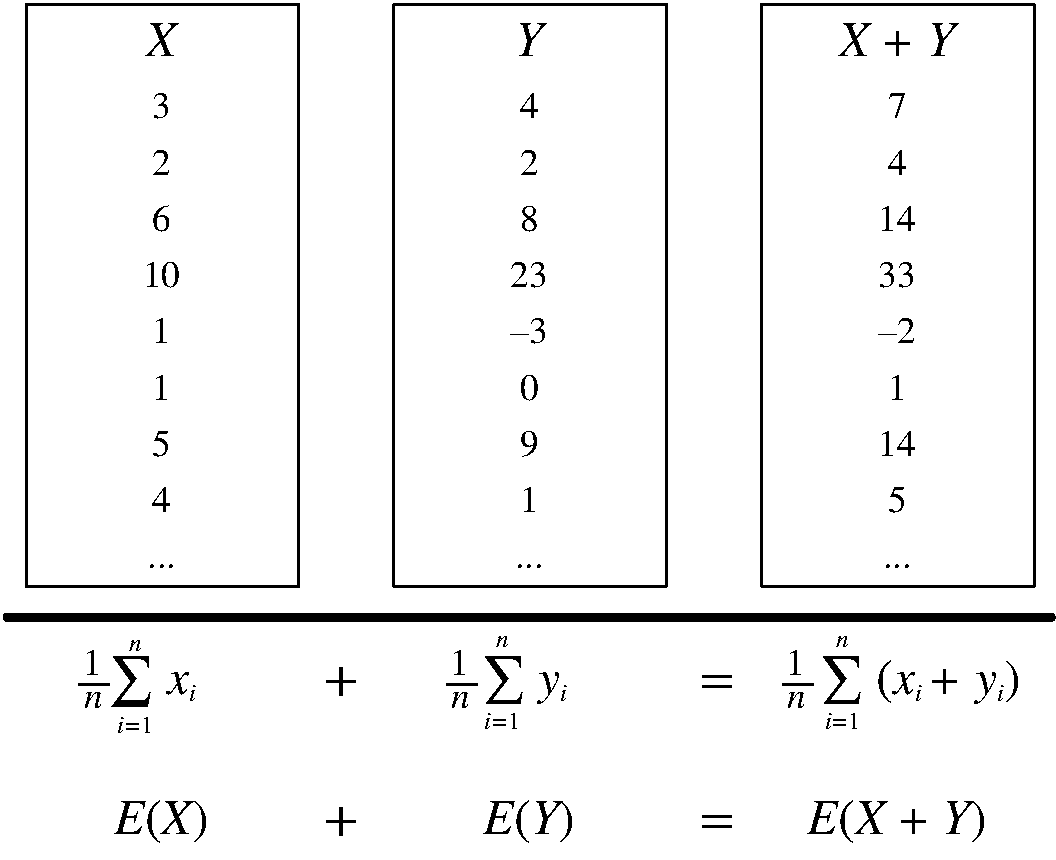
\includegraphics[width=2in]{figures/linearity.pdf}
        \end{minipage}


\item[Linearity] For any r.v.s $X$ and $Y$, and constants $a,b,c,$ 
\[E(aX + bY + c) = aE(X) + bE(Y) + c \]

\item[Same distribution implies same mean] If $X$ and $Y$ have the same distribution, then $E(X)=E(Y)$ and, more generally, 
$$E(g(X)) = E(g(Y))$$


\item[Conditional Expected Value] is defined like expectation, only conditioned on any event $A$. \begin{center}
$\ E(X | A) = \sum\limits_{x}xP(X=x | A)$
\end{center}

\end{description}

\subsection{Indicator Random Variables}
\begin{description}
\item[Indicator Random Variable] is a random variable that takes on the value 1 or 0. It is always an indicator of some event: if the event occurs, the indicator is 1; otherwise it is 0. They are useful for many problems about counting how many events of some kind occur. Write \[
I_A =
 \begin{cases}
   1 & \text{if $A$ occurs,} \\
   0 & \text{if $A$ does not occur.}
  \end{cases}
\]
Note that $I_A^2 = I_A, I_A I_B = I_{A \cap B}, $ and $I_{A \cup B} = I_A + I_B - I_A I_B$. 
\item[Distribution] $I_A \sim \Bern(p)$ where $p = P(A)$.
\item[Fundamental Bridge] The expectation of the indicator for event $A$ is the probability of event $A$: $E(I_A) = P(A)$. 
\end{description}

\subsection{Variance and Standard Deviation}
\[\var(X) = E \left(X - E(X)\right)^2 = E(X^2) - (E(X))^2\]
\[\textrm{SD}(X) = \sqrt{\var(X)}\]


\section{Continuous RVs, LOTUS,  UoU}\smallskip \hrule height 2pt \smallskip

\subsection{Continuous Random Variables (CRVs)}
\begin{description}
% \item[What is a Continuous Random Variable (CRV)?] A continuous random variable can take on any possible value within a certain interval (for example, [0, 1]), whereas a discrete random variable can only take on variables in a list of countable values (for example, all the integers, or the values 1, $\frac{1}{2}, \frac{1}{4}, \frac{1}{8}$, etc.)
% \item[Do Continuous Random Variables have PMFs?] No. The probability that a continuous random variable takes on any specific value is 0.
\item[What's the probability that a CRV is in an interval?] Take the difference in CDF values (or use the PDF as described later).
\[P(a \leq X \leq b) = P(X \leq b) - P(X \leq a) = F_X(b) - F_X(a)\]

For $X \sim \N(\mu,\sigma^2)$, this becomes
\begin{align*}
P(a\leq X\leq b)&=\Phi \left(\frac{b-\mu }{\sigma } \right) - \Phi \left( \frac{a-\mu }{\sigma } \right)
\end{align*}

\item[What is the Probability Density Function (PDF)?] The PDF $f$ is the derivative of the CDF $F$.
\[ F'(x) = f(x) \]
A PDF is nonnegative and integrates to $1$. By the fundamental theorem of calculus, to get from PDF back to CDF we can integrate:
\begin{align*} 
    F(x) &=  \int_{-\infty}^x f(t)dt  
   \end{align*}
   \begin{minipage}{\linewidth}
            \centering
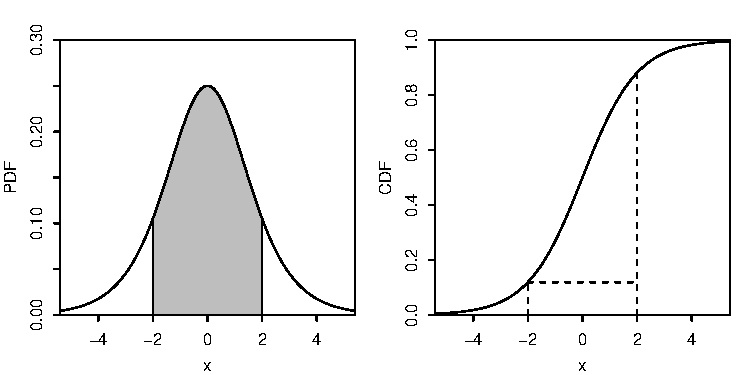
\includegraphics[width=2in]{figures/Logisticpdfcdf.pdf}
        \end{minipage}
   To find the probability that a CRV takes on a value in an interval, integrate the PDF over that interval.
      \begin{align*} 
    F(b) - F(a)  &=  \int^b_a f(x)dx
       \end{align*}
   


% Two additional properties of a PDF:  it must integrate to 1 (because the probability that a CRV falls in the interval $[-\infty, \infty]$ is 1, and the PDF must always be nonnegative.
% \[\int^\infty_{-\infty}f(x)dx \hspace{2 cm} f(x) \geq 0\]
\item[How do I find the expected value of a CRV?] Analogous to the discrete case, where you sum $x$ times the PMF, for CRVs you integrate $x$ times the PDF.
\[E(X) = \int^\infty_{-\infty}xf(x)dx \]
% Review: Expected value is \emph{linear}. This means that for \emph{any} random variables $X$ and $Y$ and any constants $a, b, c$, the following is true:
% \[E(aX + bY + c) = aE(X) + bE(Y) + c\]
\end{description}


\label{lotus}
\subsection{LOTUS}
\begin{description}
\item[Expected value of a function of an r.v.]
The expected value of $X$ is defined this way:
\[E(X) = \sum_x xP(X=x) \textnormal{ (for discrete $X$)}\]
\[E(X) = \int^\infty_{-\infty}xf(x)dx  \textnormal{ (for continuous $X$)}\]
The \textbf{Law of the Unconscious Statistician (LOTUS)} states that you can find the expected value of a \emph{function of a random variable}, $g(X)$, in a similar way, by replacing the $x$ in front of the PMF/PDF by $g(x)$ but still working with the PMF/PDF of $X$:
\[E(g(X)) = \sum_x g(x)P(X=x) \textnormal{ (for discrete $X$)}\]
\[E(g(X)) = \int^\infty_{-\infty}g(x)f(x)dx \textnormal{ (for continuous $X$)}\]
\item[What's a function of a random variable?] A function of a random variable is also a random variable. For example, if $X$ is the number of bikes you see in an hour, then $g(X) =  2X$ is the number of bike wheels you see in that hour and $h(X) = {X \choose 2} = \frac{X(X-1)}{2}$ is the number of \emph{pairs} of bikes such that you see both of those bikes in that hour.
\item[What's the point?] You don't need to know the PMF/PDF of $g(X)$ to find its expected value. All you need is the PMF/PDF of $X$. 
\end{description}

\subsection{Universality of Uniform (UoU)} When you plug any CRV into its own CDF, you get a Uniform(0,1) random variable. When you plug a Uniform(0,1) r.v.~into an inverse CDF, you get an r.v.~with that CDF. For example, let's say that a random variable $X$ has CDF
    \[ F(x) = 1 - e^{-x}, \textrm{ for $x>0$} \]
    By  UoU, if we plug $X$ into this function then we get a uniformly distributed random variable.
    \[ F(X) = 1 - e^{-X} \sim \textrm{Unif}(0,1)\]
    Similarly, if $U \sim \textrm{Unif}(0,1)$ then $F^{-1}(U)$ has CDF $F$. The key point is that {for any continuous random variable $X$, we can transform it into a Uniform random variable and back by using its CDF.}

\section{Moments and MGFs}\smallskip \hrule height 2pt \smallskip

\subsection{Moments}

Moments describe the shape of a distribution. Let $X$ have mean $\mu$ and standard deviation $\sigma$, and $Z=(X-\mu)/\sigma$ be the \emph{standardized} version of $X$. The $k$th moment of $X$ is $\mu_k = E(X^k)$ and the $k$th standardized moment of $X$ is $ m_k = E (Z^k)$.
The mean, variance,  skewness, and kurtosis are important summaries of the shape of a distribution.
    \begin{description}
        \item[Mean] $E(X) = \mu_1 $
        \item[Variance] $\var(X) = \mu_2 - \mu_1^2$
        \item[Skewness] $\textrm{Skew}(X) = m_3$
      \item[Kurtosis] $\textrm{Kurt}(X) = m_4 - 3$
    \end{description}

\subsection{Moment Generating Functions}

\begin{description}
    \item[MGF] For any random variable $X$, the function
        \[ M_X(t) = E(e^{tX}) \]
        is the \textbf{moment generating function (MGF)} of $X$, if it exists for all $t$ in some open interval containing $0$. The variable $t$ could just as well have been called $u$ or $v$. It's a bookkeeping device that lets us work with the \emph{function} $M_X$ rather than the \emph{sequence} of moments. 
                
            \item[Why is it called the Moment Generating Function?] Because the $k$th derivative of the moment generating function, evaluated at $0$, is the $k$th moment of $X$.
    \[\mu_k = E(X^k) = M_X^{(k)}(0)\]
    This is true by Taylor expansion of $e^{tX}$ since
    \[M_X(t) = E(e^{tX}) = \sum_{k=0}^\infty \frac{E(X^k)t^k}{k!} = \sum_{k=0}^\infty \frac{\mu_k t^k}{k!} \]

    \item[MGF of linear functions] If we have $Y = aX + b$, then
        \[M_Y(t) = E(e^{t(aX + b)}) =  e^{bt}E(e^{(at)X}) = e^{bt}M_X(at)\]
       
    \item[Uniqueness] \emph{If it exists, the MGF uniquely determines the distribution}. This means that for any two random variables $X$ and $Y$, they are distributed the same (their PMFs/PDFs are equal) if and only if their MGFs are equal. 
    \item[Summing Independent RVs by Multiplying MGFs.] If $X$ and $Y$ are independent, then
    \begin{align*}
        M_{X+Y}(t) &= E(e^{t(X + Y)}) = E(e^{tX})E(e^{tY}) = M_X(t) \cdot M_Y(t) 
    \end{align*}
    The MGF of the sum of two random variables is the product of the MGFs of those two random variables.
\end{description}

\section{Joint PDFs and CDFs}\smallskip \hrule height 2pt \smallskip

\subsection{Joint Distributions}
The \textbf{joint CDF} of $X$ and $Y$ is 
$$F(x,y)=P(X \leq x, Y \leq y)$$
In the discrete case, $X$ and $Y$ have a \textbf{joint PMF} 
$$p_{X,Y}(x,y) = P(X=x,Y=y).$$ In the continuous case, they have a \textbf{joint PDF}
\[f_{X,Y}(x,y) = \frac{\partial^2}{\partial x \partial y} F_{X,Y}(x,y).\]
The joint PMF/PDF must be nonnegative and sum/integrate to 1.
\begin{minipage}{\linewidth}
            \centering
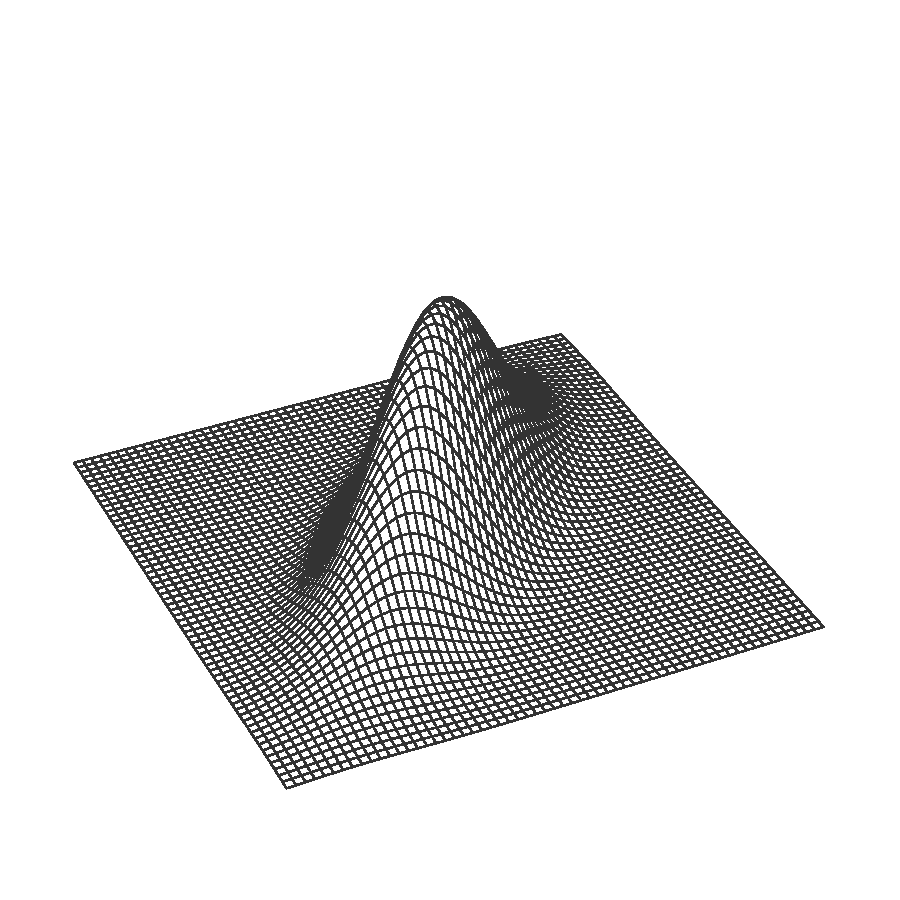
\includegraphics[width=1.0in]{figures/jointPDF.pdf}
        \end{minipage}
\subsection{Conditional Distributions}
\textbf{Conditioning and Bayes' rule for discrete r.v.s}
\[P(Y=y|X=x) = \frac{P(X=x, Y=y)}{P(X=x)} = \frac{P(X=x|Y=y)P(Y=y)}{P(X=x)}\]
\textbf{Conditioning and Bayes' rule for continuous r.v.s}
\[f_{Y|X}(y|x) = \frac{f_{X,Y}(x, y)}{f_X(x)} = \frac{f_{X|Y}(x|y)f_Y(y)}{f_X(x)}\]
\textbf{Hybrid Bayes' rule}
\[f_X(x|A) = \frac{P(A | X = x)f_X(x)}{P(A)}\]

\subsection{Marginal Distributions}
To find the distribution of one (or more) random variables from a joint PMF/PDF, sum/integrate over the unwanted random variables. \medskip

\textbf{Marginal PMF from joint PMF}
\[P(X = x) = \sum_y P(X=x, Y=y)\]
\textbf{Marginal PDF from joint PDF}
\[f_X(x) = \int_{-\infty}^\infty f_{X, Y}(x, y) dy\]


\subsection{Independence of Random Variables}
Random variables $X$ and $Y$ are independent if and only if any of the following conditions holds:
\begin{itemize}
    \itemsep -1mm
    \item Joint CDF is the product of the marginal CDFs 
    \item Joint PMF/PDF is the product of the marginal PMFs/PDFs
    \item Conditional distribution of $Y$ given $X$ is the marginal distribution of $Y$
\end{itemize}
 Write $X \independent Y$ to denote that $X$ and $Y$ are independent.

\subsection{Multivariate LOTUS}
LOTUS in more than one dimension is analogous to the 1D LOTUS.
For discrete random variables:
\[E(g(X, Y)) = \sum_x\sum_yg(x, y)P(X=x, Y=y)\]
For continuous random variables:
\[E(g(X, Y)) = \int_{-\infty}^{\infty}\int_{-\infty}^{\infty}g(x, y)f_{X,Y}(x, y)dxdy\]

\section{Covariance and Transformations}\smallskip \hrule height 2pt \smallskip

\subsection{Covariance and Correlation}
\begin{description}
\item [Covariance] is the analog of variance for two random variables.
    \[\cov(X, Y) = E\left((X - E(X))(Y - E(Y))\right) = E(XY) - E(X)E(Y)\]
    Note that 
    \[\cov(X, X) = E(X^2) - (E(X))^2 =  \var(X)\]
\item [Correlation] is a standardized version of covariance that is always between $-1$ and $1$.
    \[\corr(X, Y) = \frac{\cov(X, Y)}{\sqrt{\var(X)\var(Y)}} \]
\item [Covariance and Independence] If two random variables are independent, then they are uncorrelated. The converse is not necessarily true (e.g., consider $X \sim \N(0,1)$ and $Y=X^2$).
    \begin{align*}
    	X \independent Y &\longrightarrow \cov(X, Y) = 0 \longrightarrow E(XY) = E(X)E(Y)
    \end{align*}
%, except in the case of Multivariate Normal, where uncorrelated \emph{does} imply independence.
\item [Covariance and Variance]  The variance of a sum can be found by
    \begin{align*}
        %\cov(X, X) &= \var(X) \\
        \var(X + Y) &= \var(X) + \var(Y) + 2\cov(X, Y) \\
        \var(X_1 + X_2 + \dots + X_n ) &= \sum_{i = 1}^{n}\var(X_i) + 2\sum_{i < j} \cov(X_i, X_j)
    \end{align*}
    If $X$ and $Y$ are independent then they have covariance $0$, so
    \[X \independent Y \Longrightarrow \var(X + Y) = \var(X) + \var(Y)\]
    If $X_1, X_2, \dots, X_n$ are identically distributed and have the same covariance relationships (often by \textbf{symmetry}), then 
    \[\var(X_1 + X_2 + \dots + X_n ) = n\var(X_1) + 2{n \choose 2}\cov(X_1, X_2)\]
\item [Covariance Properties]  For random variables $W, X, Y, Z$ and constants $a, b$:
    \begin{align*}
    	\cov(X, Y) &= \cov(Y, X) \\
        \cov(X + a, Y + b) &= \cov(X, Y) \\
        \cov(aX, bY) &= ab\cov(X, Y) \\
        \cov(W + X, Y + Z) &= \cov(W, Y) + \cov(W, Z) + \cov(X, Y)\\
        &\quad + \cov(X, Z)
    \end{align*}
\item [Correlation is location-invariant and scale-invariant] For any constants $a,b,c,d$ with $a$ and $c$ nonzero,
    \begin{align*}
        \corr(aX + b, cY + d) &= \corr(X, Y) 
    \end{align*}
\end{description}

\subsection{Transformations}
\begin{description}
    \label{one variable transformations}
    \item[One Variable Transformations] Let's say that we have a random variable $X$ with PDF $f_X(x)$, but we are also interested in some function of $X$. We call this function $Y = g(X)$. Also let $y=g(x)$. If $g$ is differentiable and strictly increasing (or strictly decreasing), then the PDF of $Y$ is
    \[f_Y(y) = f_X(x)\left|\frac{dx}{dy}\right| =  f_X(g^{-1}(y))\left|\frac{d}{dy}g^{-1}(y)\right|\]
    The derivative of the inverse transformation is called the \textbf{Jacobian}.


     \item[Two Variable Transformations] Similarly, let's say we know the joint PDF of $U$ and $V$ but are also interested in the random vector $(X, Y)$ defined by $(X, Y) = g(U, V)$. Let 
       $$  \frac{\partial (u,v)}{\partial (x,y)}  = \begin{pmatrix} 
              \frac{\partial u}{\partial x} &  \frac{\partial u}{\partial y} \\
           \frac{\partial v}{\partial x} & \frac{\partial v}{\partial y}   \\
        \end{pmatrix}$$
     be the \textbf{Jacobian matrix}. If the entries in this matrix exist and are continuous, and the determinant of the matrix is never $0$, then
     \[f_{X,Y}(x, y) = f_{U,V}(u,v) \left|\left|   \frac{\partial (u,v)}{\partial (x,y)}\right| \right| \]
   The inner bars tells us to take the matrix's determinant, and the outer bars tell us to take the absolute value.  In a $2 \times 2$ matrix, 
     \[ \left| \left|
     \begin{array}{ccc}
         a & b \\
         c & d
     \end{array}
     \right| \right| = |ad - bc|\]

\end{description}

\label{convolutions}
\subsection{Convolutions}
\begin{description}
    \item[Convolution Integral] If you want to find the PDF of the sum of two independent CRVs $X$ and $Y$, you can do the following integral:
        \[f_{X+Y}(t)=\int_{-\infty}^\infty f_X(x)f_Y(t-x)dx\]
    \item[Example] Let $X,Y \sim \N(0,1)$ be i.i.d. Then for each fixed $t$,\[f_{X+Y}(t)=\int_{-\infty}^\infty \frac{1}{\sqrt{2\pi}}e^{-x^2/2} \frac{1}{\sqrt{2\pi}}e^{-(t-x)^2/2} dx\]
By completing the square and using the fact that a Normal PDF integrates to $1$, this works out to $f_{X+Y}(t)$ being the $\N(0,2)$ PDF.
\end{description}

\section{Poisson Process}\smallskip \hrule height 2pt \smallskip

\begin{description}
\item[Definition] We have a \textbf{Poisson process} of rate $\lambda$ arrivals per unit time if the following conditions hold:
\begin{enumerate}
    \item The number of arrivals in a time interval of length $t$ is $\Pois(\lambda t)$.
    \item Numbers of arrivals in disjoint time intervals are independent.
\end{enumerate}
For example, the numbers of arrivals in the time intervals $[0,5]$, $(5,12),$ and $[13,23)$ are independent with $\Pois(5\lambda), \Pois(7\lambda), \Pois(10\lambda)$ distributions, respectively.
\begin{minipage}{\linewidth}
            \centering
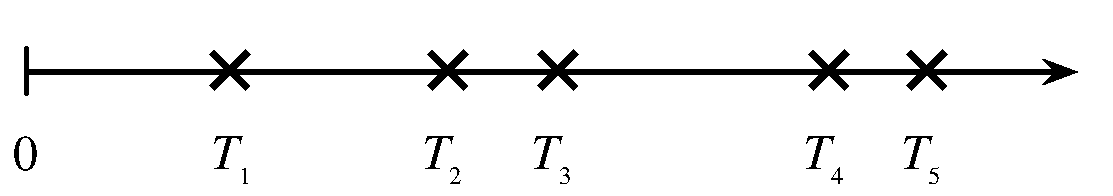
\includegraphics[width=2in]{figures/pp.pdf}
        \end{minipage}
       
\item[Count-Time Duality]  Consider a Poisson process of emails arriving in an inbox at rate $\lambda$ emails per hour. Let $T_n$ be the time of arrival of the $n$th email (relative to some starting time $0$) and $N_t$ be the number of emails that arrive in $[0,t]$. Let's find the distribution of $T_1$. The event $T_1 > t$, the event that you have to wait more than $t$ hours to get the first email, is the same as the event $N_t = 0$, which is the event that there are no emails in the first $t$ hours. So
\[P(T_1 > t) = P(N_t = 0) = e^{-\lambda t} \longrightarrow P(T_1 \leq t) = 1 - e^{-\lambda t}\]
Thus we have $T_1 \sim \Expo(\lambda)$. By the memoryless property and similar reasoning, the interarrival times between emails are i.i.d.~$\Expo(\lambda)$, i.e., the differences $T_n - T_{n-1}$ are i.i.d.~$\Expo(\lambda)$.
\end{description}

\section{Order Statistics}\smallskip \hrule height 2pt \smallskip
\begin{description}
    \item[Definition] Let's say you have $n$ i.i.d.~r.v.s $X_1, X_2,\dots, X_n$. If you arrange them from smallest to largest, the $i$th element in that list is the $i$th order statistic, denoted $X_{(i)}$. So $X_{(1)}$ is the smallest in the list and $X_{(n)}$ is the largest in the list. \smallskip
    
     Note that the order statistics are \emph{dependent}, e.g., learning $X_{(4)} = 42$ gives us the information that $X_{(1)},X_{(2)},X_{(3)}$ are $\leq 42$ and $X_{(5)},X_{(6)},\dots,X_{(n)}$ are $\geq 42$.
    \item[Distribution]  Taking $n$ i.i.d. random variables $X_1, X_2, \dots, X_n$ with CDF $F(x)$ and PDF $f(x)$, the CDF and PDF of $X_{(i)}$ are:
        \[F_{X_{(i)}}(x) = P (X_{(i)} \leq x) = \sum_{k=i}^n {n \choose k} F(x)^k(1 - F(x))^{n - k}\]
    \[f_{X_{(i)}}(x) = n{n - 1 \choose i - 1}F(x)^{i-1}(1 - F(x))^{n-i}f(x)\]
%    \item[Universality of the Uniform] Let $X_1,X_2,\dots,X_n$ be i.i.d.~CRVs with CDF $F$, and let $U_j=F(X_j)$. By UoU, $U_1,U_2,\dots,U_n$ are i.i.d.~$\Unif(0,1)$. Since $F$ is increasing, $F(X_{(1)}) \leq F(X_{(2)}) \leq \dots \leq F(X_{(n)})$, so $U_{(j)} = F(X_{(j)})$.
    \item[Uniform Order Statistics]  The $j$th order statistic of i.i.d.~$U_1,\dots,U_n \sim \Unif(0,1)$ is $U_{(j)} \sim \Beta(j, n - j + 1)$.
\end{description}


\section{Conditional Expectation}\smallskip \hrule height 2pt \smallskip
\begin{description}
    \item[Conditioning on an Event] We can find $E(Y|A)$, the expected value of $Y$ given that event $A$ occurred. A very important case is when $A$ is the event $X=x$. Note that $E(Y|A)$ is a \emph{number}. For example: 
    \begin{itemize}
    \item The expected value of a fair die roll, given that it is prime, is $\frac{1}{3} \cdot 2 + \frac{1}{3} \cdot 3 + \frac{1}{3} \cdot 5 = \frac{10}{3}$.
    \item Let $Y$ be the number of successes in $10$ independent Bernoulli trials with probability $p$ of success. Let $A$ be the event that the first $3$ trials are all successes. Then
    $$E(Y|A) = 3 + 7p$$
    since the number of successes among the last $7$ trials is $\Bin(7,p)$. 
        \item Let $T \sim \Expo(1/10)$ be how long you have to wait until the shuttle comes. Given that you have already waited $t$ minutes, the expected additional waiting time is 10 more minutes, by the memoryless property. That is, $E(T|T>t) = t + 10$.
    \end{itemize}
\end{description}
        \scalebox{0.85}{
                        \setlength{\extrarowheight}{7pt}
            \begin{tabular}{ccc}
                  \textbf{Discrete $Y$} & \textbf{Continuous $Y$} \\
            \toprule
            $E(Y) = \sum_y yP(Y=y)$ & $E(Y) =\int_{-\infty}^\infty yf_Y(y)dy$ \\
           % $E(Y|X=x) = \sum_y yP(Y=y|X=x)$ & $E(Y|X=x) =\int_{-\infty}^\infty yf_{Y|X}(y|x)dy$ \\
            $E(Y|A) = \sum_y yP(Y=y|A)$ & $E(Y|A) = \int_{-\infty}^\infty yf(y|A)dy$ \\ 
            \bottomrule
            \end{tabular}
        }
        \medskip
\begin{description}
    \item[Conditioning on a Random Variable]  We can also find $E(Y|X)$, the expected value of $Y$ given the random variable $X$. This is \emph{a function of the random variable $X$}. It is \emph{not} a number except in certain special cases such as if $X \independent Y$. To find $E(Y|X)$, find $E(Y|X = x)$ and then plug in $X$ for $x$. For example:
    \begin{itemize}
    \item If $E(Y|X=x) = x^3+5x$, then $E(Y|X) = X^3 + 5X$.
    \item Let $Y$ be the number of successes in $10$ independent Bernoulli trials with probability $p$ of success and $X$ be the number of successes among the first $3$ trials. Then $E(Y|X)=X+7p$.
    \item Let $X \sim \N(0,1)$ and $Y=X^2$. Then $E(Y|X=x) = x^2$ since if we know $X=x$ then we know $Y=x^2$. And $E(X|Y=y) = 0$ since if we know $Y=y$ then we know $X = \pm \sqrt{y}$, with equal probabilities (by symmetry). So $E(Y|X)=X^2, E(X|Y)=0$.  
    \end{itemize} 
    
        \item[Properties of Conditional Expectation] \quad
    \begin{enumerate}
        \item $E(Y|X) = E(Y)$ if $X \independent Y$
        \item $E(h(X)W|X) = h(X)E(W|X)$ (\textbf{taking out what's known}) \\
        In particular, $E(h(X)|X) = h(X)$.
        \item $E(E(Y|X)) = E(Y)$ (\textbf{Adam's Law}, a.k.a.~Law of Total Expectation)
    \end{enumerate}

    \item[Adam's Law (a.k.a.~Law of Total Expectation)]  can also be written in a way that looks analogous to LOTP. For any events $A_1, A_2, \dots, A_n$ that partition the sample space, 
        \begin{align*}
        E(Y) &= E(Y|A_1)P(A_1) + \dots + E(Y|A_n)P(A_n)
    \end{align*}
    For the special case where the partition is $A, A^c$, this says
        \begin{align*}
            E(Y) &= E(Y|A)P(A) + E(Y|A^c)P(A^c)
    \end{align*}

    \item[Eve's Law (a.k.a.~Law of Total Variance)] \quad
    \[\var(Y) = E(\var(Y|X)) + \var(E(Y|X))\]
\end{description}


\section{MVN, LLN, CLT}\smallskip \hrule height 2pt \smallskip

\subsection{Law of Large Numbers (LLN)}
Let $X_1, X_2, X_3 \dots$ be i.i.d.~with mean $\mu$. The \textbf{sample mean} is $$\bar{X}_n = \frac{X_1 + X_2 + X_3 + \dots + X_n}{n}$$ The \textbf{Law of Large Numbers} states that as $n \to \infty$, $\bar{X}_n \to \mu$ with probability $1$. For example, in flips of a coin with probability $p$ of Heads, let $X_j$ be the indicator of the $j$th flip being Heads.  Then LLN says the proportion of Heads converges to $p$ (with probability $1$).

\subsection{Central Limit Theorem (CLT)}
\subsubsection{Approximation using CLT}
We use $\dot{\,\sim\,}$ to denote \emph{is approximately distributed}. We can use the \textbf{Central Limit Theorem} to approximate the distribution of a random variable $Y=X_1+X_2+\dots+X_n$ that is a sum of $n$ i.i.d. random variables $X_i$. Let  $E(Y) = \mu_Y$ and $\var(Y) = \sigma^2_Y$. The CLT says
\[Y \dot{\,\sim\,} \N(\mu_Y, \sigma^2_Y)\]
If the $X_i$ are i.i.d.~with mean $\mu_X$ and variance $\sigma^2_X$, then $\mu_Y = n \mu_X$ and $\sigma^2_Y = n \sigma^2_X$. For the sample mean $\bar{X}_n$, the CLT says
\[ \bar{X}_n = \frac{1}{n}(X_1 + X_2 + \dots + X_n) \dot{\,\sim\,} \N(\mu_X, \sigma^2_X/n) \]


\subsubsection{Asymptotic Distributions using CLT}

We use $\xrightarrow{D}$ to denote \emph{converges in distribution to} as $n  \to \infty$. The CLT says that if we standardize the sum $X_1 + \dots + X_n$  then the distribution of the sum converges to $\N(0,1)$ as $n \to \infty$:
\[\frac{1}{\sigma\sqrt{n}} (X_1 + \dots + X_n - n\mu_X) \xrightarrow{D} \N(0, 1)\]
In other words, the CDF of the left-hand side goes to the standard Normal CDF, $\Phi$. In terms of the sample mean, the CLT says
\[ \frac{\sqrt{n} (\bar{X}_n - \mu_X)}{\sigma_X} \xrightarrow{D} \N(0, 1)\]

\section{Markov Chains}\smallskip \hrule height 2pt \smallskip

\subsection{Definition}
\begin{minipage}{\linewidth}
            \centering
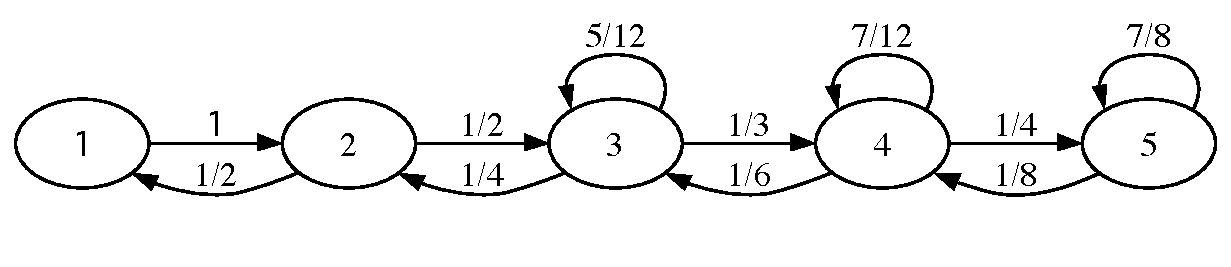
\includegraphics[width=2.3in]{figures/chainA.pdf}
        \end{minipage}
A Markov chain is a random walk in a \textbf{state space}, which we will assume is finite, say $\{1, 2, \dots, M\}$. We let $X_t$ denote which element of the state space the walk is visiting at time $t$. The Markov chain is the sequence of random variables tracking where the walk is at all points in time, $X_0, X_1, X_2, \dots$. By definition, a Markov chain must satisfy the \textbf{Markov property}, which says that if you want to predict where the chain will be at a future time, if we know the present state then the entire past history is irrelevant.  \emph{Given the present, the past and future are conditionally independent}. In symbols,
\[P(X_{n+1} = j | X_0 = i_0, X_1 = i_1, \dots, X_n = i) = P(X_{n+1} = j | X_n = i)\]
\subsection{State Properties}
A state is either recurrent or transient.
\begin{itemize}
\item If you start at a \textbf{recurrent state}, then you will always return back to that state at some point in the future.  \textmusicalnote \emph{You can check-out any time you like, but you can never leave.}  \textmusicalnote
\item Otherwise you are at a \textbf{transient state}. There is some positive probability that once you leave you will never return. \textmusicalnote \emph{You don't have to go home, but you can't stay here.} \textmusicalnote
\end{itemize}
A state is either periodic or aperiodic.
\begin{itemize}
\item If you start at a \textbf{periodic state} of period $k$, then the GCD of  the possible numbers of steps it would take to return back is  $k>1$.
\item Otherwise you are at an \textbf{aperiodic state}. The GCD of  the possible numbers of steps it would take to return back is 1.
\end{itemize}


\subsection{Transition Matrix}
Let the state space be $\{1,2,\dots,M\}$. The transition matrix $Q$ is the $M \times M$ matrix where element $q_{ij}$ is the probability that the chain goes from state $i$ to state $j$ in one step:
\[q_{ij} = P(X_{n+1} = j | X_n = i)\]

To find the probability that the chain goes from state $i$ to state $j$ in exactly $m$ steps, take the $(i, j)$ element of $Q^m$.
\[q^{(m)}_{ij} = P(X_{n+m} = j | X_n = i)\]
If $X_0$ is distributed according to the row vector PMF $\vec{p}$, i.e., $p_j = P(X_0 = j)$, then the PMF of $X_n$ is $\vec{p}Q^n$.



\subsection{Chain Properties}
A chain is \textbf{irreducible} if you can get from anywhere to anywhere. If a chain (on a finite state space) is irreducible, then all of its states are recurrent. A chain is \textbf{periodic} if any of its states are periodic, and is \textbf{aperiodic} if none of its states are periodic. In an irreducible chain, all states have the same period. \medskip

A chain is \textbf{reversible} with respect to $\vec{s}$ if $s_iq_{ij} = s_jq_{ji}$ for all $i, j$.  Examples of reversible chains include any chain with $q_{ij} = q_{ji}$, with $\vec{s} = (\frac{1}{M}, \frac{1}{M}, \dots, \frac{1}{M})$, and random walk on an undirected network.

\subsection{Stationary Distribution}

Let us say that the vector $\vec{s} = (s_1, s_2, \dots, s_M)$ be a PMF  (written as a row vector). We will call $\vec{s}$ the \textbf{stationary distribution} for the chain if $\vec{s}Q = \vec{s}$. As a consequence, if $X_t$ has the stationary distribution, then all future $X_{t+1}, X_{t + 2}, \dots$ also have the stationary distribution. \\

\smallskip

For irreducible, aperiodic chains, the stationary distribution exists, is unique, and $s_i$ is the long-run probability of a chain being at state $i$. The expected number of steps to return to $i$ starting from $i$ is $1/s_i$.

\smallskip

 To find the stationary distribution, you can solve the matrix equation $(Q' - I){\vec{s}\,}'= 0$. The stationary distribution is uniform if the columns of $Q$ sum to 1.

\smallskip

\textbf{Reversibility Condition Implies Stationarity}  If you have a PMF $\vec{s}$ and a Markov chain with transition matrix $Q$, then $s_iq_{ij} = s_jq_{ji}$ for all states $i, j$ implies that $\vec{s}$ is stationary.

\subsection{Random Walk on an Undirected Network}
 \begin{minipage}{\linewidth}
            \centering
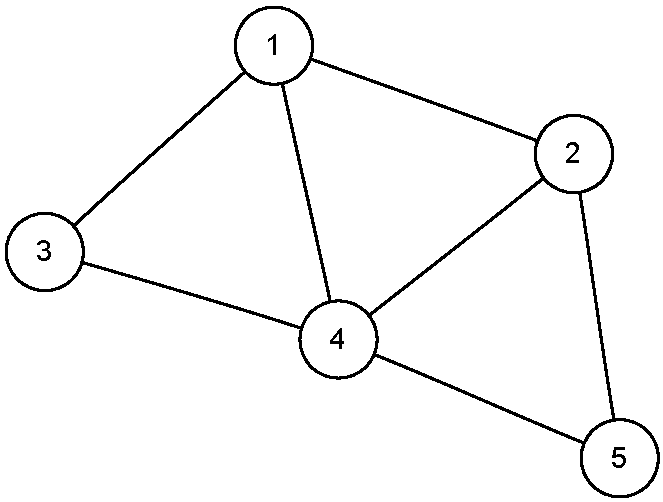
\includegraphics[width=1.6in]{figures/network1.pdf}
        \end{minipage}
\medskip

If you have a collection of \textbf{nodes}, pairs of which can be connected by undirected \textbf{edges}, and a Markov chain is run by going from the current node to a uniformly random node that is connected to it by an edge, then  this is a random walk on an undirected network. The stationary distribution of this chain is proportional to the \textbf{degree sequence} (this is the sequence of degrees, where the degree of a node is how many edges are attached to it). For example, the stationary distribution of random walk on the network shown above is proportional to $(3,3,2,4,2)$, so it's $(\frac{3}{14}, \frac{3}{14}, \frac{3}{14}, \frac{4}{14}, \frac{2}{14})$. 

\section{Continuous Distributions}\smallskip \hrule height 2pt \smallskip

\subsection{Uniform Distribution} Let us say that $U$ is distributed $\Unif(a, b)$. We know the following:
\begin{description}
    \item[Properties of the Uniform] For a Uniform distribution, the probability of a draw from any interval within the support is proportional to the length of the interval. See  \emph{Universality of Uniform} and \emph{Order Statistics} for other properties.
     \item[Example] William throws darts really badly, so his darts are uniform over the whole room because they're equally likely to appear anywhere. William's darts have a Uniform distribution on the surface of the room. The Uniform is the only distribution where the probability of hitting in any specific region is proportional to the length/area/volume of that region, and where the density of occurrence in any one specific spot is constant throughout the whole support.
%     \item[PDF and CDF (top is Unif(0, 1), bottom is Unif(a, b))]  
% \begin{eqnarray*}
% %\Unif(0, 1)
%   %\hspace{.7 in}
%    f(x) = \left\{
%      \begin{array}{lr}
%        1 & x \in [0, 1] \\
%        0 &  x \notin [0, 1]
%      \end{array}
%    \right.
%    %\hspace{.95 in}
%    F(x) = \left\{
%      \begin{array}{lr}
%        0 & x < 0 \\
%        x & x \in [0, 1] \\
%        1 &  x > 1
%      \end{array}
%    \right.\\
% %\Unif(a, b)
%   %\hspace{.65 in}
%    f(x) = \left\{
%      \begin{array}{lr}
%        \frac{1}{b-a} & x \in [a, b] \\
%        0 &  x \notin [a, b]
%      \end{array}
%    \right.
%    %\hspace{.75 in}
%    F(x) = \left\{
%      \begin{array}{lr}
%        0 & x < a \\
%        \frac{x-a}{b-a} & x \in [a, b] \\
%        1 &  x > b
%      \end{array}
%    \right. 
% \end{eqnarray*}


    
\end{description}

\subsection{Normal Distribution} Let us say that $X$ is distributed $\N(\mu, \sigma^2)$. We know the following:
\begin{description}
    \item[Central Limit Theorem] The Normal distribution is ubiquitous because of the Central Limit Theorem, which states that the sample mean of i.i.d.~r.v.s will approach a Normal distribution as the sample size grows, regardless of the initial distribution.
    \item[Location-Scale Transformation] Every time we shift a Normal r.v.~(by adding a constant) or rescale a Normal (by multiplying by a constant), we change it to another Normal r.v. For any Normal $X \sim \N(\mu, \sigma^2)$, we can transform it to the standard $\N(0, 1)$ by the following transformation:
    \[Z= \frac{X - \mu}{\sigma} \sim \N(0, 1) \]
%    \item[Example] Heights are normal. Measurement error is normal. By the central limit theorem, the sampling average from a population is also normal.
    \item[Standard Normal] The Standard Normal, $Z \sim \N(0, 1)$, has mean $0$ and variance $1$. Its CDF is denoted by $\Phi$.
\end{description}

\subsection{Exponential Distribution}

Let us say that $X$ is distributed $\Expo(\lambda)$. We know the following:
\begin{description}
    \item[Story] You're sitting on an open meadow right before the break of dawn, wishing that airplanes in the night sky were shooting stars, because you could really use a wish right now. You know that shooting stars come on average every 15 minutes, but a shooting star is  not ``due" to come just because you've waited so long. Your waiting time is memoryless;  the additional time until the next shooting star comes does not depend on how long you've waited already.
    
    \item[Example] The waiting time until the next shooting star is distributed $\Expo(4)$ hours. Here $\lambda=4$ is the \textbf{rate parameter}, since shooting stars arrive at a rate of $1$ per $1/4$ hour on average. The expected time until the next shooting star is $1/\lambda = 1/4$ hour.
    
    \item[Expos as a rescaled Expo(1)]
        \[Y \sim \Expo(\lambda) \rightarrow X = \lambda Y \sim \Expo(1)\]
     
%     \item[PDF and CDF] The PDF and CDF of a Exponential is:
% \[f(x) = \lambda e^{-\lambda x}, x \in [0, \infty)\]
% \[F(x) = P(X \leq x) = 1 - e^{-\lambda x}, x \in [0, \infty)\]
    
    \item[Memorylessness] The Exponential Distribution is the only continuous memoryless distribution. The memoryless property says that for $X \sim \Expo(\lambda)$ and any positive numbers $s$ and $t$,
    \[P(X > s + t | X > s) = P(X > t)\]
Equivalently,
    \[X - a | (X > a) \sim \Expo(\lambda)\]
    For example, a product with an $\Expo(\lambda)$ lifetime is always ``as good as new" (it doesn't experience wear and tear). Given that the product has survived $a$ years, the additional time that it will last is still $\Expo(\lambda)$. 

%    Example - If waiting for the bus is distributed exponentially with $\lambda = 6$, no matter how long you've waited so far, the expected additional waiting time until the bus arrives is always $\frac{1}{6}$, or 10 minutes. The distribution of time from now to the arrival is always the same, no matter how long you've waited.

    \item[Min of Expos] If we have independent $X_i \sim \Expo(\lambda_i)$, then $\min(X_1, \dots, X_k) \sim \Expo(\lambda_1 + \lambda_2 + \dots + \lambda_k)$. 
    \item[Max of Expos] If we have i.i.d.~$X_i \sim \Expo(\lambda)$, then $\max(X_1, \dots, X_k)$ has the same distribution as $Y_1+Y_2+\dots+Y_k$, where $Y_j \sim \Expo(j\lambda)$ and the $Y_j$ are independent.     
\end{description}

\subsection{Gamma Distribution}
\begin{minipage}{\linewidth}
            \centering
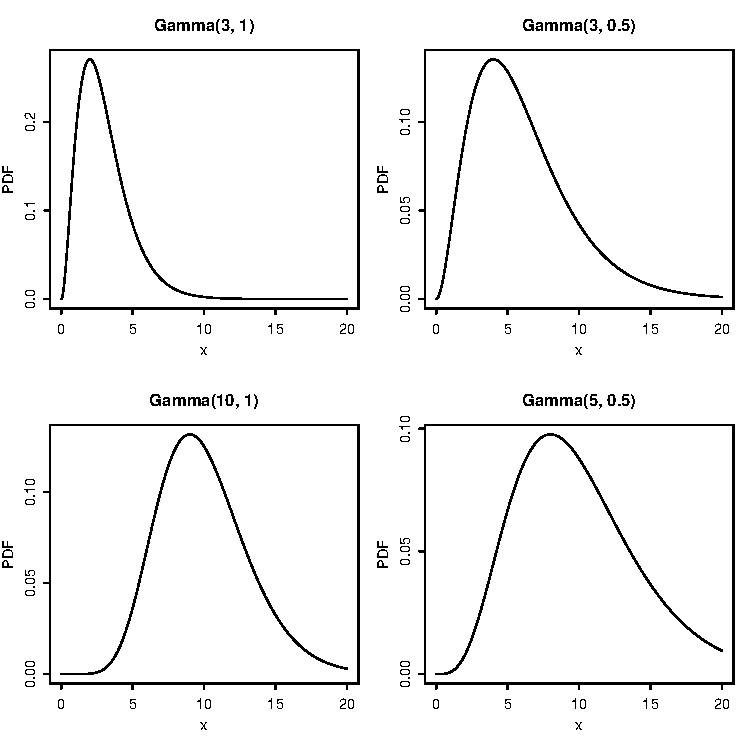
\includegraphics[width=1.9in]{figures/gammapdfs.pdf}
        \end{minipage}
\medskip
Let us say that $X$ is distributed $\Gam(a, \lambda)$. We know the following:
\begin{description}
    \item[Story] You sit waiting for shooting stars, where the waiting time for a star is distributed $\Expo(\lambda)$. You want to see $n$ shooting stars before you go home. The total waiting time for the $n$th shooting star is $\Gam(n,\lambda)$.
    \item[Example]  You are at a bank, and there are 3 people ahead of you. The serving time for each person is Exponential with mean $2$ minutes. Only one person at a time can be served. The distribution of your waiting time until it's your turn to be served is $\Gam(3, \frac{1}{2})$.
%     \item[PDF] The PDF of a Gamma is:
% \begin{eqnarray*}
% f(x) = \frac{1}{\Gamma(a)}(\lambda x)^ae^{-\lambda x}\frac{1}{x},
% \hspace{.1 in}
% x \in [0, \infty)
% \end{eqnarray*}
    % \item[Properties and Representations]

\end{description}

\subsection{Beta Distribution}
\begin{minipage}{\linewidth}
            \centering
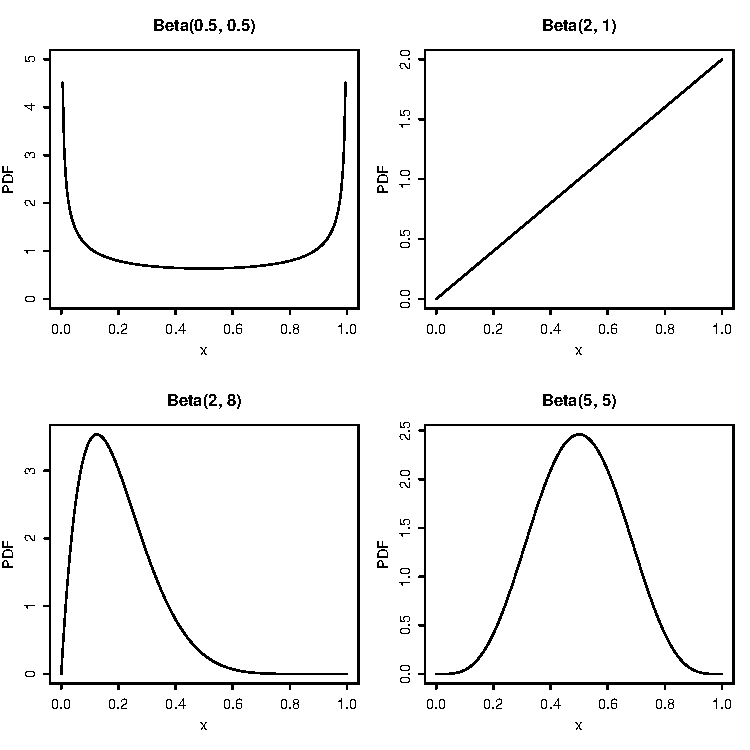
\includegraphics[width=1.9in]{figures/Betapdfs.pdf}
        \end{minipage}
\medskip

\begin{description}

\item[Conjugate Prior of the Binomial] In the Bayesian approach to statistics, parameters are viewed as random variables, to reflect our uncertainty. The \emph{prior} for a parameter is its distribution before observing data. The \emph{posterior}  is the distribution for the parameter after observing data. Beta is the \emph{conjugate} prior of the Binomial because if you have a Beta-distributed prior on $p$ in a Binomial, then the posterior distribution on $p$ given the Binomial data is also Beta-distributed. Consider the following two-level model:
    \begin{align*}
        X|p &\sim \Bin(n, p) \\
        p &\sim \Beta(a, b)
    \end{align*}
Then after observing  $X = x$, we get the posterior distribution
\[p|(X=x) \sim \Beta(a + x, b + n - x) \]

\item[Order statistics of the Uniform] See \emph{Order Statistics}.
\item[Beta-Gamma relationship] If $X \sim \Gam(a, \lambda)$, $Y \sim \Gam(b, \lambda)$, with $X \independent Y$ then
    \begin{itemize}
    	\item $\frac{X}{X + Y} \sim \Beta(a, b)$
    	\item $X + Y \independent \frac{X}{X + Y}$
    \end{itemize}
    This is known as the \textbf{bank--post office result}.
\end{description}


% \[E(X) = \frac{a}{\lambda},  Var(X) = \frac{a}{\lambda^2}\]
% \[X \sim G(a, \lambda),  Y \sim G(b, \lambda),  X \independent Y \rightarrow  X + Y \sim G(a + b, \lambda), \frac{X}{X + Y} \independent X + Y \]
% \[X \sim \Gam(a, \lambda) \rightarrow X = X_1 + X_2 + ... + X_a \textnormal{ for $X_i$ i.i.d. $\Expo(\lambda)$} \]
% \[\Gam(1, \lambda) \sim \Expo(\lambda) \]


\subsection{$\chi^2$ (Chi-Square) Distribution}

Let us say that $X$ is distributed $\chi^2_n$. We know the following:
\begin{description}
    \item[Story] A Chi-Square($n$) is the sum of the squares of $n$ independent standard Normal r.v.s.
    %\item[Example]  The sum of squared errors are distributed $\chi^2_n$
%     \item[PDF] The PDF of a $\chi^2_1$ is:
% \begin{eqnarray*}
% f(w) = \frac{1}{\sqrt{2\pi w}}e^{-w/2},
% w \in [0, \infty)
% \end{eqnarray*}
    \item[Properties and Representations]
\[X \textrm{ is distributed as } Z_1^2 + Z_2^2 + \dots + Z_n^2 \textrm{ for i.i.d.~$Z_i \sim \N(0,1)$}\]
\[X \sim \Gam(n/2,1/2)\]
\end{description}

\section{Discrete Distributions} \smallskip \hrule height 2pt \smallskip

\subsection{Distributions for four sampling schemes}
\begin{center}
    \begin{tabular}{ccc}
        ~ & \textbf{Replace} & \textbf{No Replace}  \\
    \midrule
        \textbf{Fixed \# trials ($n$)} & Binomial & HGeom \\ 
        ~ & (Bern if $n = 1$) & ~ \\ 
        \textbf{Draw until $r$ success} & NBin & NHGeom \\ 
        ~ & (Geom if $r = 1$) & ~\\ \bottomrule
    \end{tabular}
\end{center}

\subsection{Bernoulli Distribution} The Bernoulli distribution is the simplest case of the Binomial distribution, where we only have one trial ($n=1$). Let us say that X is distributed \Bern($p$). We know the following:
\begin{description}
    \item[Story] A trial is performed with probability $p$ of ``success", and $X$ is the indicator of success: $1$ means success, $0$ means failure.
        \item[Example] Let $X$ be the indicator of Heads for a fair coin toss. Then $X \sim \Bern(\frac{1}{2})$. Also, $1-X  \sim \Bern(\frac{1}{2})$ is the indicator of Tails.
        %     \item[PMF.] The probability mass function of a Bernoulli is:
% \[P(X = x) = p^x(1-p)^{1-x}\]
% or simply
% \[P(X = x) = \begin{cases} p, & x = 1 \\ 1-p, & x = 0 \end{cases}\]
\end{description}

\subsection{Binomial Distribution} 
\begin{minipage}{\linewidth}
            \centering
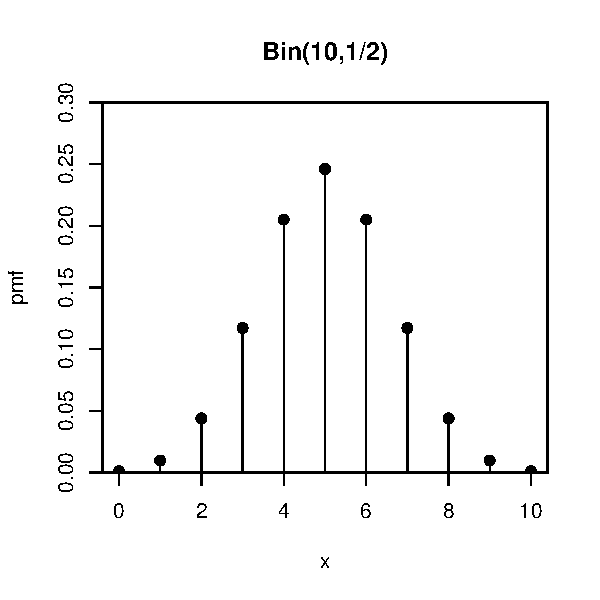
\includegraphics[width=1.3in]{figures/Bin10,05.pdf}
        \end{minipage}

Let us say that $X$ is distributed \Bin($n,p$). We know the following:
\begin{description}
    \item[Story] $X$ is the number of ``successes" that we will achieve in $n$ independent trials, where each trial is either a success or a failure, each with the same probability $p$ of success. We can also write $X$ as a sum of multiple independent $\Bern(p)$ random variables. Let $X \sim \Bin(n, p)$ and $X_j \sim \Bern(p)$, where all of the Bernoullis are independent. Then
        \[X = X_1 + X_2 + X_3 + \dots + X_n\]
    \item[Example] If Jeremy Lin makes 10 free throws and each one independently has a $\frac{3}{4}$ chance of getting in, then the number of free throws he makes is distributed  \Bin($10,\frac{3}{4}$).
    %     \item[PMF] The probability mass function of a Binomial is:
% \[P(X = x) = {n  \choose x} p^x(1-p)^{n-x}\]
\item[Properties] Let $X \sim \Bin(n,p), Y \sim \Bin(m,p)$ with $X \independent Y$.
\begin{itemize}
\item \textbf{Redefine success} $n-X \sim \Bin(n,1-p)$
\item \textbf{Sum} $X+Y \sim \Bin(n+m,p)$
\item \textbf{Conditional} $X|(X+Y=r) \sim \HGeom(n,m,r)$
 \item \textbf{Binomial-Poisson Relationship} $\Bin(n, p)$ is approximately  $\Pois(\lambda)$ if $p$ is small.
   \item \textbf{Binomial-Normal Relationship} $\Bin(n, p)$ is approximately $\N(np,np(1-p))$ if $n$ is large and $p$ is not near $0$ or $1$.
  \end{itemize}
\end{description}

\subsection{Geometric Distribution} Let us say that $X$ is distributed $\Geom(p)$. We know the following:
\begin{description}
    \item[Story] $X$ is the number of ``failures" that we will achieve before we achieve our first success. Our successes have probability $p$.
    \item[Example] If each pokeball we throw has probability  $\frac{1}{10}$ to catch Mew, the number of failed pokeballs will be distributed $\Geom(\frac{1}{10})$.
%     \item[PMF] With $q = 1-p$, the probability mass function of a Geometric is:
% \[P(X = k) = q^kp\]
\end{description}

\subsection{First Success Distribution} Equivalent to the Geometric distribution, except that it includes the first success in the count. This is 1 more than the number of failures. If $X \sim \textnormal{FS}(p)$ then $E(X) = 1/p$.


\subsection{Negative Binomial Distribution} Let us say that $X$ is distributed $\NBin(r, p)$. We know the following:
\begin{description}
    \item[Story] $X$ is the number of ``failures" that we will have before we achieve our $r$th success. Our successes have probability $p$.
    \item[Example] Thundershock has 60\% accuracy and can faint a wild Raticate in 3 hits. The number of misses before Pikachu faints Raticate with Thundershock is distributed $\NBin(3, 0.6)$.
%     \item[PMF] With $q = 1-p$, the probability mass function of a Negative Binomial is:
% \[P(X = n) = {n+r - 1 \choose r -1}p^rq^n\]
\end{description}

\subsection{Hypergeometric Distribution} Let us say that $X$ is distributed $\Hypergeometric(w, b, n)$. We know the following:
\begin{description}
    \item[Story] In a population of $w$ desired objects and  $b$ undesired objects, $X$ is the number of ``successes" we will have in a draw of $n$ objects, without replacement. The draw of $n$ objects is assumed to be a \textbf{simple random sample} (all sets of $n$ objects are equally likely).
    \item[Examples] Here are some HGeom examples.
    \begin{itemize}
    \item Let's say that we have only $b$ Weedles (failure) and $w$ Pikachus (success) in Viridian Forest. We encounter $n$ Pokemon in the forest, and $X$ is the number of Pikachus in our encounters. 
    \item The number of Aces in a 5 card hand.
    \item You have $w$ white balls and $b$ black balls, and you draw $n$ balls. You will draw $X$ white balls.
    \item You have $w$ white balls and $b$ black balls, and you draw $n$ balls without replacement. The number of white balls in your sample is $\HGeom(w,b,n)$; the number of black balls is $\HGeom(b,w,n)$. 
    \item \textbf{Capture-recapture} A forest has $N$ elk, you capture $n$ of them, tag them, and release them. Then you recapture a new sample of size $m$. How many tagged elk are now in the new sample? $\HGeom(n,N-n,m)$
    \end{itemize} 
%    \item[PMF] The probability mass function of a Hypergeometric:
%\[P(X = k) = \frac{{w \choose k}{b \choose n-k}}{{w + b \choose n}}\]
\end{description}

\subsection{Poisson Distribution} Let us say that $X$ is distributed $\Pois(\lambda)$. We know the following:
\begin{description}
    \item[Story] There are rare events (low probability events) that occur many different ways (high possibilities of occurences) at an average rate of $\lambda$ occurrences per unit space or time. The number of events that occur in that unit of space or time is $X$.
    
    \item[Example] A certain busy intersection has an average of 2 accidents per month. Since an accident is a low probability event that can happen many different ways, it is reasonable to model the number of accidents in a month at that intersection as $\Pois(2)$. Then the number of accidents that happen in two months at that intersection is distributed $\Pois(4)$.
    
    \item[Properties]
Let $X \sim \Pois(\lambda_1)$ and $Y \sim \Pois(\lambda_2)$, with $X \independent Y$.

\begin{enumerate}
    \item \textbf{Sum} $X + Y \sim \Pois(\lambda_1 + \lambda_2)$
    \item \textbf{Conditional} $X | (X + Y = n) \sim \Bin\left(n, \frac{\lambda_1}{\lambda_1 + \lambda_2}\right)$
    \item \textbf{Chicken-egg} If there are $Z \sim \Pois(\lambda)$ items and we randomly and independently ``accept" each item with probability $p$, then the number of accepted items $Z_1 \sim \Pois(\lambda p)$, and the number of rejected items $Z_2 \sim \Pois(\lambda (1-p))$, and $Z_1 \independent Z_2$.
\end{enumerate}
    
%     \item[PMF] The PMF of a Poisson is:
% \[P(X = k) = \frac{e^{-\lambda}\lambda^k}{k!}\]
\end{description}


\section{Multivariate Distributions} \smallskip \hrule height 2pt \smallskip


\subsection{Multinomial Distribution}
    Let us say that the vector $\vec{X} = (X_1, X_2, X_3, \dots, X_k) \sim \textnormal{Mult}_k(n, \vec{p})$  where $\vec{p} = (p_1, p_2, \dots, p_k)$.
\begin{description}
    \item[Story]  We have $n$ items, which can fall into any one of the $k$ buckets independently with the probabilities $\vec{p} = (p_1, p_2, \dots, p_k)$.
    \item[Example]  Let us assume that every year, 100 students in the Harry Potter Universe are randomly and independently sorted into one of four houses with equal probability. The number of people in each of the houses is distributed $\Mult_4$(100, $\vec{p}$), where $\vec{p} = (0.25, 0.25, 0.25, 0.25)$.
        Note that $X_1 + X_2 + \dots + X_4 = 100$, and they are dependent.
    \item[Joint PMF]  For $n = n_1 + n_2 + \dots + n_k$,
        \[P(\vec{X} = \vec{n}) =  \frac{n!}{n_1!n_2!\dots n_k!}p_1^{n_1}p_2^{n_2}\dots p_k^{n_k}\]
    \item[Marginal PMF, Lumping, and Conditionals]
    Marginally, $X_i \sim \Bin(n,p_i)$ since we can define ``success" to mean category $i$. If you lump together multiple categories in a Multinomial, then it is still Multinomial. For example, $X_i + X_j \sim \Bin(n, p_i + p_j)$ for $i \neq j$ since we can define ``success" to mean being in category $i$ or $j$. Similarly, if $k=6$ and we lump categories 1-2 and lump categories 3-5, then
        \[ (X_1+X_2,X_3+X_4+X_5,X_6) \sim \Mult_3(n, (p_1+p_2, p_3 + p_4+p_5,p_6))\]
        Conditioning on some $X_j$ also still gives a Multinomial:
        \[X_1, \dots, X_{k-1} | X_k = n_k \sim \Mult_{k-1}\left(n - n_k, \left(\frac{p_1}{1 - p_k}, \dots, \frac{p_{k-1}}{1 - p_k}\right)\right)\]
    \item[Variances and Covariances]  We have  $X_i \sim \Bin(n, p_i)$ marginally, so $\var(X_i) = np_i(1-p_i)$. Also, $\cov(X_i, X_j) = -np_ip_j$ for $i \neq j$.
    \end{description}
    
\subsection{Multivariate Uniform Distribution}
See the univariate Uniform for stories and examples. For the 2D Uniform on some region, probability is proportional to area. Every point in the support has equal density, of value $\frac{1}{\textnormal{area of region}}$. For the 3D Uniform, probability is proportional to volume.

\subsection{Multivariate Normal (MVN) Distribution}
A  vector $\vec{X} = (X_1, X_2, \dots, X_k)$ is  Multivariate Normal if every linear combination is Normally distributed, i.e., $t_1X_1 + t_2X_2 + \dots + t_kX_k$ is Normal for any constants $t_1, t_2, \dots, t_k$. The parameters of the Multivariate Normal are the \textbf{mean vector} $\vec{\mu} = (\mu_1, \mu_2, \dots, \mu_k)$ and the \textbf{covariance matrix} where the $(i, j)$ entry is $\cov(X_i, X_j)$. 

\begin{description}
\item[Properties] The Multivariate Normal has the following properties.
\begin{itemize}
\item Any subvector is also MVN.
\item If any two elements within an MVN are uncorrelated, then they are independent.
\item The joint PDF of a Bivariate Normal $(X,Y)$ with $\N(0,1)$ marginal distributions and correlation $\rho \in (-1,1)$ is 
$$  f_{X,Y}(x,y) = \frac{1}{2 \pi \tau} \exp{\left(-\frac{1}{2 \tau^2} (x^2+y^2-2 \rho xy)\right)},$$
with $\tau = \sqrt{1-\rho^2}.$ 
\end{itemize}
\end{description}

\section{Distribution Properties} \smallskip \hrule height 2pt \smallskip
\subsection{Important CDFs}
\begin{description}
   \item[Standard Normal] $\Phi$
    \item[Exponential($\lambda$)] $F(x) = 1 - e^{-\lambda x}, \textrm{ for } x \in (0, \infty)$
    \item[Uniform(0,1)] $F(x) = x, \textrm{ for } x \in (0, 1)$
\end{description}

\subsection{Convolutions of Random Variables}
A convolution of $n$ random variables is simply their sum. For the following results, let $X$ and $Y$ be \emph{independent}.
\begin{enumerate}
    \item  $X \sim \Pois(\lambda_1)$, $Y \sim \Pois(\lambda_2)$ $\longrightarrow X + Y \sim \Pois(\lambda_1 + \lambda_2)$
    \item  $X \sim \Bin(n_1, p)$, $Y \sim \Bin(n_2, p)$ $\longrightarrow X + Y \sim \Bin(n_1 + n_2, p)$. $\Bin(n,p)$ can be thought of as a sum of i.i.d.~$\Bern(p)$ r.v.s.
    \item  $X \sim \Gam(a_1, \lambda)$, $Y \sim \Gam(a_2, \lambda)$ $\longrightarrow  X + Y \sim\Gam(a_1 + a_2, \lambda)$.  $\Gam(n,\lambda)$ with $n$ an integer can  be thought of as a sum of i.i.d.~Expo($\lambda$) r.v.s.
    \item  $X \sim \NBin(r_1, p)$, $Y \sim \NBin(r_2, p)$ $\longrightarrow  X + Y \sim\NBin(r_1 + r_2, p)$. $\NBin(r,p)$ can  be thought of as a sum of i.i.d.~Geom($p$) r.v.s.
    \item  $X \sim \N(\mu_1, \sigma_1^2)$, $Y \sim \N(\mu_2, \sigma_2^2)$  $\longrightarrow  X + Y \sim \N(\mu_1 + \mu_2, \sigma_1^2 + \sigma_2^2)$
\end{enumerate}

\subsection{Special Cases of Distributions}
\begin{enumerate}
    \item $\Bin(1, p) \sim \Bern(p)$
    \item $\Beta(1, 1) \sim \Unif(0, 1)$
    \item $\Gam(1, \lambda) \sim \Expo(\lambda)$
    \item $\chi^2_n \sim \Gam\left(\frac{n}{2}, \frac{1}{2}\right)$
    \item $\NBin(1, p) \sim \Geom(p)$
\end{enumerate}

\subsection{Inequalities}

\begin{enumerate}
\item \textbf{Cauchy-Schwarz} $|E(XY)| \leq \sqrt{E(X^2)E(Y^2)}$
\item \textbf{Markov} $P(X \geq a) \leq \frac{E|X|}{a}$ for $a>0$
\item \textbf{Chebyshev} $P(|X - \mu| \geq a) \leq \frac{\sigma^2}{a^2}$ for $E(X)=\mu, \var(X) = \sigma^2$
\item \textbf{Jensen} $E(g(X)) \geq g(E(X))$ for $g$ convex; reverse if $g$ is concave
\end{enumerate}


\section{Formulas} \smallskip \hrule height 2pt \smallskip
\subsection{Geometric Series}
\[ 1 + r + r^2 + \dots + r^{n-1} = \sum_{k=0}^{n-1} r^k = \frac{1 - r^n}{1 -r} \]
\[ 1 + r + r^2 + \dots = \frac{1}{1-r} \textnormal{ if $|r|<1$} \]

\subsection{Exponential Function ($e^x$)}
\[ e^x = \sum_{n=0}^\infty \frac{x^n}{n!}= 1 + x + \frac{x^2}{2!} + \frac{x^3}{3!} + \dots = \lim_{n \rightarrow \infty} \left( 1 + \frac{x}{n} \right)^n \]

\subsection{Gamma and Beta Integrals}
You can sometimes solve complicated-looking integrals by pattern-matching to a gamma or beta integral:
\[ \int_0^\infty x^{t-1}e^{-x}\, dx = \Gamma(t) \hspace{1 cm} \int_0^1 x^{a - 1}(1-x)^{b-1}\, dx = \frac{\Gamma(a)\Gamma(b)}{\Gamma(a + b)} \]
Also, $\Gamma(a+1) = a \Gamma(a)$, and $\Gamma(n) = (n - 1)!$ if $n$ is a positive integer. 
\subsection{Euler's Approximation for Harmonic Sums}
\[ 1 + \frac{1}{2} + \frac{1}{3} + \dots + \frac{1}{n} \approx \log n + 0.577 \dots\]
\subsection{Stirling's Approximation for Factorials}
\[ n! \approx \sqrt{2\pi n}\left(\frac{n}{e}\right)^n\]

\section{Miscellaneous Definitions} \smallskip \hrule height 2pt \smallskip

\begin{description}
\item[Medians and Quantiles] Let $X$ have CDF $F$. Then $X$ has median $m$ if $F(m) \geq 0.5$ and $P(X \geq m) \geq 0.5$. For $X$ continuous, $m$ satisfies $F(m)=1/2$. In general, the $a$th quantile of $X$ is $\min \{x: F(x)\geq a\}$; the median is the case $a=1/2$.
\item[log] Statisticians generally use $\log$ to refer to natural log (i.e., base $e$).
\item[i.i.d r.v.s] Independent, identically-distributed random variables.

\end{description}

\section{Example Problems} \smallskip \hrule height 2pt \smallskip
Contributions from Sebastian Chiu

\subsection{Calculating Probability}
A textbook has $n$ typos, which are randomly scattered amongst its $n$ pages, independently. You pick a random page. What is the probability that it has no typos? \textbf{Answer:} There is a $\left( 1 - \frac{1}{n} \right)$ probability that any specific typo isn't on your page, and thus a $\boxed{\left( 1 - \frac{1}{n} \right)^n}$ probability that there are no typos on your page. For $n$ large, this is approximately $e^{-1} = {1/e}$.

\subsection{Linearity and Indicators (1)} In a group of $n$ people, what is the expected number of distinct birthdays (month and day)? What is the expected number of birthday matches? \textbf{Answer:} Let $X$ be the number of distinct birthdays and $I_j$ be the indicator for the $j$th day being represented. \[E(I_j) = 1-P(\textnormal{no one born on day }j) = 1 - \left(364/365\right)^n\] By linearity, $\boxed{E(X) = 365\left(1-(364/365\right)^n)}$. 
Now let $Y$ be the number of birthday matches and $J_i$ be the indicator that the $i$th pair of people have the same birthday. The probability that any two specific people share a birthday is $1/365$, so $\boxed{E(Y) = \binom{n}{2} / 365}$. 

\subsection{Linearity and Indicators (2)}
\emph{This problem is commonly known as the \textbf{hat-matching problem}}. There are $n$ people at a party, each with hat. At the end of the party, they each leave with a random hat. What is the expected number of people who leave with the right hat? \textbf{Answer:} Each hat has a $1/n$ chance of going to the right person. By linearity, the average number of hats that go to their owners is $\boxed{n(1/n) = 1}$.

\subsection{Linearity and First Success}
\emph{This problem is commonly known as the \textbf{coupon collector problem}}.
There are $n$ coupon types. At each draw, you get a uniformly random coupon type. What is the expected number of coupons needed until you have a complete set? \textbf{Answer:} Let $N$ be the number of coupons needed; we want $E(N)$. Let $N = N_1 + \dots + N_n$, where $N_1$ is the draws to get our first new coupon, $N_2$ is the \emph{additional} draws needed to draw our second new coupon and so on. By the story of the First Success, $N_2 \sim \textnormal{FS}((n-1)/n)$ (after collecting first coupon type, there's $(n-1)/n$ chance you'll get something new). Similarly, $N_3 \sim \textnormal{FS}((n-2)/n)$, and $N_j \sim \textnormal{FS}((n-j+1)/n)$. By linearity,
\[E(N) = E(N_1) + \dots + E(N_n) = \frac{n}{n} + \frac{n}{n-1} + \dots + \frac{n}{1} = \boxed{n\sum^n_{j=1} \frac{1}{j}}\]
This is approximately $n (\log(n) + 0.577)$ by Euler's approximation.

\subsection{Orderings of i.i.d. random variables}
I call 2 UberX's and 3 Lyfts at the same time. If the time it takes for the rides to reach me are i.i.d., what is the probability that all the Lyfts will arrive first? \textbf{Answer:} Since the arrival times of the five cars are i.i.d., all $5!$ orderings of the arrivals are equally likely. There are $3!2!$ orderings that involve the Lyfts arriving first, so the probability that the Lyfts arrive first is $\boxed{\frac{3!2!}{5!} = 1/10}$. Alternatively, there are ${5 \choose 3}$ ways to choose 3 of the 5 slots for the Lyfts to occupy, where each of the choices are equally likely. One of these choices has all 3 of the Lyfts arriving first, so the probability is $\boxed{1 / {5 \choose 3} = 1/10}$.

\subsection{Expectation of Negative Hypergeometric}
What is the expected number of cards that you draw before you pick your first Ace in a shuffled deck (not counting the Ace)?
\textbf{Answer:} Consider a non-Ace. Denote this to be card $j$. Let $I_j$ be the indicator that card $j$ will be drawn before the first Ace. Note that $I_j=1$ says that  $j$ is before all 4 of the Aces in the deck. The probability that this occurs is $1/5$ by symmetry. Let $X$ be the number of cards drawn before the first Ace. Then $X = I_1 + I_2 + ... + I_{48}$, where each indicator corresponds to one of the 48 non-Aces. Thus, \[E(X) = E(I_1) + E(I_2) + ... + E(I_{48}) = 48/5 = \boxed{9.6}.\]

\subsection{Minimum and Maximum of RVs}
What is the CDF of the maximum of $n$ independent Unif(0,1) random variables? \textbf{Answer:} Note that for r.v.s $X_1,X_2,\dots,X_n$, 
\[ P(\min(X_1, X_2, \dots, X_n) \geq a) = P(X_1 \geq a, X_2 \geq a, \dots, X_n \geq a) \] Similarly, \[ P(\max(X_1, X_2, \dots, X_n) \leq a) = P(X_1 \leq a, X_2 \leq a, \dots, X_n \leq a) \] We will use this principle to find the CDF of $U_{(n)}$, where $U_{(n)} = \max(U_1, U_2, \dots, U_n)$ and $U_i \sim \Unif(0, 1)$ are i.i.d.
\begin{align*}
P(\max(U_1, U_2, \dots, U_n) \leq a)
&= P(U_1 \leq a, U_2 \leq a, \dots, U_n \leq a) \\
&= P(U_1 \leq a)P(U_2 \leq a)\dots P(U_n \leq a) \\
&= \boxed{a^n}
\end{align*}
for $0<a<1$ (and the CDF is $0$ for $a \leq 0$ and $1$ for $a \geq 1$).

\subsection{Pattern-matching with $e^x$ Taylor series}
For $X \sim \Pois(\lambda)$, find $\displaystyle E\bigg{(}\frac{1}{X+1}\bigg{)}$. \textbf{Answer:} By LOTUS,
\[E\left(\frac{1}{X+1}\right) = \displaystyle\sum_{k=0}^\infty \frac{1}{k+1} \frac{e^{-\lambda}\lambda^k}{k!} = \frac{e^{-\lambda}}{\lambda}\sum_{k=0}^\infty \frac{\lambda^{k+1}}{(k+1)!} = \boxed{\frac{e^{-\lambda}}{\lambda}(e^\lambda-1)}\]

\subsection{Adam's Law and Eve's Law}
William really likes speedsolving Rubik's Cubes. But he's pretty bad at it, so sometimes he fails. On any given day, William will attempt $N \sim \Geom(s)$ Rubik's Cubes. Suppose each time, he has probability $p$ of solving the cube, independently. Let $T$ be the number of Rubik's Cubes he solves during a day. Find the mean and variance of $T$. \textbf{Answer:} Note that $T|N \sim \Bin(N,p)$. So by Adam's Law, \[E(T) = E(E(T|N)) = E(Np) = \boxed{\displaystyle\frac {p (1-s)}{s}}\] Similarly, by Eve's Law, we have that \begin{align*}
    \var(T) &= E(\var(T|N)) + \var(E(T|N)) =  E(Np(1-p)) + \var(Np)\\&= \frac{p(1-p)(1-s)}{s} +  \frac{p^2(1-s)}{s^2} = \boxed{\frac{p(1-s)(p+s(1-p))}{s^2}}
    \end{align*}

%\subsection{MGF -- Distribution Matching}
%(Continuing the Rubik's Cube question above) Find the MGF of $T$. What is the name of this distribution and its parameter(s)? \textbf{Answer:}
%
%    By Adam's Law, we have  \begin{align*} E(e^{tT}) &= E(E(e^{tT}|N)) =E((pe^t + q)^N) = s\sum_{n=0}^\infty(pe^t + 1-p)^n(1-s)^n \\&=\frac{s}{1-(1-s)(pe^t+1-p)} =\frac{s}{s+(1-s)p-(1-s)pe^t}
%    \end{align*}
%    
%    Intuitively, we would expect that $T$ is distributed Geometrically since $T$ is just a filtered version of $N$, which itself is Geometrically distributed. The MGF of $X\sim\Geom(\theta)$ is \[E(e^{tX}) = \displaystyle\frac{\theta}{1-(1-\theta) e^t}\]
%    
%    So, we would want to try to get our MGF into this form to identify what $\theta$ is. Taking our original MGF, it would appear that dividing by $s+(1-s)p$ would allow us to do this. Therefore, we have that \begin{center}
%    $E(e^{tT}) = \displaystyle\frac{s}{s+(1-s)p - (1-s)pe^t} = \frac{\frac{s}{s+(1-s)p}}{1-\frac{(1-s)p}{s+(1-s)p}e^t}$
%    \end{center}
%    
%    By pattern-matching, it thus follows that $\boxed{T \sim \Geom(\theta)}$ where \[\boxed{\theta = \displaystyle\frac{s}{s+(1-s)p}}\]

\subsection{MGF -- Finding Moments}
Find $E(X^3)$ for $X \sim \Expo(\lambda)$ using the MGF of $X$. \textbf{Answer:} The MGF of an $\Expo(\lambda)$ is $M(t) = \frac{\lambda}{\lambda-t}$. To get the third moment, we can take the third derivative of the MGF and evaluate at $t=0$: 
\[\boxed{E(X^3) = \frac{6}{\lambda^3}}\]
But a much nicer way to use the MGF here is via pattern recognition: note that $M(t)$ looks like it came from a geometric series:
\[\frac{1}{1-\frac{t}{\lambda}} = \sum^{\infty}_{n=0} \left(\frac{t}{\lambda}\right)^n = \sum^{\infty}_{n=0} \frac{n!}{\lambda^n} \frac{t^n}{n!}\] The coefficient of $\frac{t^n}{n!}$ here is the $n$th moment of $X$, so we have $E(X^n) = \frac{n!}{\lambda^n}$ for all nonnegative integers $n$. 

\subsection{Markov chains (1)}
Suppose $X_n$ is a two-state Markov chain with transition matrix \[
Q = \bordermatrix{~ & 0 & 1 \cr
                  0 & 1-\alpha & \alpha \cr
                  1 & \beta & 1-\beta \cr}
\] Find the stationary distribution $\vec{s} = (s_0, s_1)$ of $X_n$ by solving $\vec{s} Q = \vec{s}$, and show that the chain is reversible with respect to $\vec{s}$. \textbf{Answer:} The equation $\vec{s}Q = \vec{s}$ says  that \[s_0 = s_0(1-\alpha) + s_1 \beta \textnormal{ and } s_1 = s_0(\alpha) + s_0(1-\beta)\] By solving this system of linear equations, we have \[\boxed{\vec{s} = \displaystyle\bigg{(}\frac{\beta}{\alpha+\beta}, \frac{\alpha}{\alpha+\beta}\bigg{)}}\] To show that the chain is reversible with respect to $\vec{s}$, we must show $s_i q_{ij} = s_j q_{ji}$ for all $i, j$. This is done if we can show $s_0 q_{01} = s_1 q_{10}$. And indeed, \[s_0  q_{01}  = \frac{\alpha\beta}{\alpha+\beta} = s_1 q_{10}\]

\subsection{Markov chains (2)}
William and Sebastian play a modified game of Settlers of Catan, where every turn they randomly move the robber (which starts on the center tile) to one of the adjacent hexagons.

% hex grid code modified from http://tex.stackexchange.com/questions/61429/how-to-draw-a-hexagonal-grid-with-numbers-in-the-cells
\begin{center}
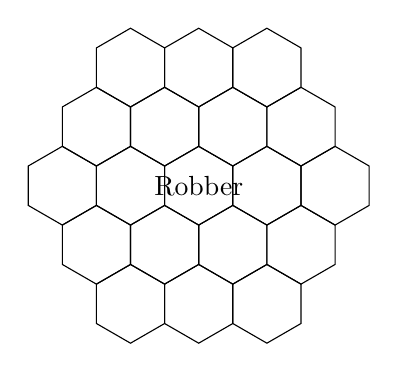
\begin{tikzpicture} [hexa/.style= {shape=regular polygon,regular polygon sides=6,minimum size=1cm, draw,inner sep=0,anchor=south,rotate=30}]
\foreach \j in {0,...,2}{%
\pgfmathsetmacro\end{2+\j} 
  \foreach \i in {0,...,\end}{%
  \node[hexa] (h\i;\j) at ({(\i-\j/2)*sin(60)},{\j*0.75}) {};}  }      
\node [circle,minimum size=1cm] at (h2;2) {Robber};
\foreach \j in {0,...,1}{%
  \pgfmathsetmacro\end{3-\j} 
  \foreach \i in {0,...,\end}{%
  \pgfmathtruncatemacro\k{\j+2}  
  \node[hexa] (h\i;\k) at ({(\i+\j/2-0.5)*sin(60)},{2.25+\j*0.75}) {};}  } 
\end{tikzpicture}
\end{center}

\begin{enumerate}[label=(\alph*)]
    \item Is this Markov chain irreducible? Is it aperiodic? \textbf{Answer:} $\boxed{\textnormal{Yes to both.}}$ The Markov chain is irreducible because it can get from anywhere to anywhere else. The Markov chain is  aperiodic because the robber can return back to a square in $2, 3, 4, 5, \dots$ moves, and the GCD of those numbers is $1$.
        \item What is the stationary distribution of this Markov chain? \textbf{Answer:} Since this is a random walk on an undirected graph, the stationary distribution is proportional to the degree sequence. The degree for the corner pieces is 3, the degree for the edge pieces is 4, and the degree for the center pieces is 6. To normalize this degree sequence, we divide by its sum. The sum of the degrees is $6(3) + 6(4) + 7(6) = 84$. Thus the stationary probability of being on a corner is $3/84 = 1/28$, on an edge is $4/84 =  1/21$, and in the center is $6/84 = 1/14$.
    \item What fraction of the time will the robber be in the center tile in this game, in the long run? \textbf{Answer:} By the above, $\boxed{1/14}$.
    \item What is the expected amount of moves it will take for the robber to return to the center tile? \textbf{Answer:} Since this chain is irreducible and aperiodic, to get the expected time to return we can just invert the stationary probability. Thus on average it will take $\boxed{14}$ turns for the robber to return to the center tile.
\end{enumerate}


\section{Problem-Solving Strategies} \smallskip \hrule height 2pt \smallskip

Contributions from Jessy Hwang, Yuan Jiang, Yuqi Hou
\begin{enumerate}
\item \textbf{Getting started.} Start by \emph{defining relevant events and random variables}. (``Let $A$ be the event that I pick the fair coin''; ``Let $X$ be the number of successes.'') Clear notion is important for clear thinking! Then decide what it is that you're supposed to be finding, in terms of your notation (``I want to find $P(X=3|A)$''). Think about what type of object your answer should be (a number? A random variable? A PMF? A PDF?) and what it should be in terms of.

\emph{Try simple and extreme cases}. To make an abstract experiment more concrete, try \emph{drawing a picture} or making up numbers that could have happened. Pattern recognition: does the structure of the problem resemble something we've seen before?
\item \textbf{Calculating probability of an event.} Use counting principles if the naive definition of probability applies. Is the probability of the complement easier to find? Look for symmetries. Look for something to condition on, then apply Bayes' Rule or the Law of Total Probability. 
\item \textbf{Finding the distribution of a random variable.} First make sure you need the full distribution not just the mean (see next item). Check the \emph{support} of the random variable: what values can it take on? Use this to rule out distributions that don't fit.  Is there a \emph{story} for one of the named distributions that fits the problem at hand?  Can you write the random variable as a function of an r.v. with a known distribution, say $Y = g(X)$?
\item \textbf{Calculating expectation.} If it has a named distribution, check out the table of distributions. If it's a function of an r.v. with a named distribution, try LOTUS. If it's a count of something, try breaking it up into indicator r.v.s. If you can condition on something natural, consider using Adam's law. 
\item \textbf{Calculating variance.} Consider independence, named distributions, and LOTUS. If it's a count of something, break it up into a sum of indicator r.v.s. If it's a sum, use properties of covariance. If you can condition on something natural, consider using Eve's Law.
\item \textbf{Calculating $E(X^2)$.}  Do you already know $E(X)$ or $\var(X)$? Recall that $\var(X) = E(X^2) - (E(X))^2$. Otherwise try LOTUS.
\item \textbf{Calculating covariance.} Use the properties of covariance. If you're trying to find the covariance between two components of a Multinomial distribution, $X_i, X_j$, then the covariance is $-np_ip_j$ for $i \neq j$.
\item \textbf{Symmetry.} If $X_1,\dots,X_n$ are i.i.d., consider using symmetry.
\item \textbf{Calculating probabilities of orderings.} Remember that all $n!$ ordering of i.i.d.~continuous random variables $X_1,\dots,X_n$ are equally likely.
\item \textbf{Determining independence.} There are several equivalent definitions. Think about simple and extreme cases to see if you can find a counterexample.
\item \textbf{Do a painful integral.} If your integral looks painful, see if you can write your integral in terms of a known PDF (like Gamma or Beta), and use the fact that PDFs integrate to $1$?
\item \textbf{Before moving on.} Check some simple and extreme cases, check whether the answer seems plausible, check for biohazards.\end{enumerate}


\section{Biohazards} \smallskip \hrule height 2pt \smallskip

Contributions from Jessy Hwang

\begin{enumerate} 
\item \textbf{Don't misuse the naive definition of probability.}   When answering ``What is the probability that in a group of 3 people, no two have the same birth month?'', it is \emph{not} correct to treat the people as indistinguishable balls being placed into 12 boxes, since that assumes the list of birth months \{January, January, January\} is just as likely as the list \{January, April, June\}, even though the latter is six times more likely. \\ 
\item \textbf{Don't confuse unconditional, conditional, and joint probabilities.}  In applying $P(A|B) = \frac{P(B|A)P(A)}{P(B)}$, it is \emph{not} correct to say ``$P(B) = 1$ because we know  $B$ happened''; $P(B)$ is the \emph{prior} probability of $B$. Don't confuse $P(A|B)$ with $P(A,B)$. \\
\item \textbf{Don't assume independence without justification.}  In the matching problem, the probability that card 1 is a match and card 2 is a match is not $1/n^2$.  Binomial and Hypergeometric are often confused; the trials are independent in the Binomial story and dependent in the Hypergeometric story. \\
\item \textbf{Don't forget to do sanity checks.} Probabilities must be between $0$ and $1$. Variances must be $\geq 0$. Supports must make sense. PMFs must sum to $1$. PDFs must integrate to $1$. \\
\item \textbf{Don't confuse random variables, numbers, and events.}  Let $X$ be an r.v. Then $g(X)$ is an r.v. for any function $g$. In particular, $X^2$, $|X|$, $F(X)$, and $I_{X>3}$ are r.v.s. $P(X^2 < X | X \geq 0), E(X), \var(X), $ and $g(E(X))$ are numbers. $X = 2$ and $F(X) \geq -1$ are events. It does not make sense to write $\int_{-\infty}^\infty F(X) dx$, because $F(X)$ is a random variable. It does not make sense to write $P(X)$, because $X$ is not an event. \\
\item \textbf{Don't confuse a random variable with its distribution.}  To get the PDF of $X^2$, you can't just square the PDF of $X$. The right way is to use transformations. To get the PDF of $X + Y$, you can't just add the PDF of $X$ and the PDF of $Y$. The right way is to compute the \hyperref[convolutions]{convolution}.
\item \textbf{Don't pull non-linear functions out of expectations.} $E(g(X))$ does not equal $g(E(X))$ in general. The St. Petersburg paradox is an extreme example.  See also Jensen's inequality. The right way to find $E(g(X))$ is with \hyperref[lotus]{LOTUS}.
\end{enumerate}

\vspace{1.5in}

\section{Distributions in R} \smallskip \hrule height 2pt \smallskip

\bigskip

\begin{center}
\begin{tabular}{cc}
\hline
\textbf{Command} & \textbf{What it does} \\
\hline
\texttt{help(distributions)} & shows documentation on distributions\\
\texttt{dbinom(k,n,p)} & PMF $P(X=k)$ for $X \sim \Bin(n,p)$\\
\texttt{pbinom(x,n,p)} & CDF $P(X \leq x)$ for $X \sim \Bin(n,p)$\\
\texttt{qbinom(a,n,p)} &   $a$th quantile for $X \sim \Bin(n,p)$\\
\texttt{rbinom(r,n,p)} &  vector of $r$ i.i.d.~$\Bin(n,p)$ r.v.s\\
\texttt{dgeom(k,p)} & PMF $P(X=k)$ for $X \sim \Geom(p)$\\
\texttt{dhyper(k,w,b,n)} & PMF $P(X=k)$ for $X \sim \HGeom(w,b,n)$\\
\texttt{dnbinom(k,r,p)} & PMF $P(X=k)$ for $X \sim \NBin(r,p)$\\
\texttt{dpois(k,r)} & PMF $P(X=k)$ for $X \sim \Pois(r)$\\
\texttt{dbeta(x,a,b)} & PDF $f(x)$ for $X \sim \Beta(a,b)$\\
\texttt{dchisq(x,n)} & PDF $f(x)$ for $X \sim \chi^2_n$\\
\texttt{dexp(x,b)} & PDF $f(x)$ for $X \sim \Expo(b)$\\
\texttt{dgamma(x,a,r)} & PDF $f(x)$ for $X \sim \Gam(a,r)$\\
\texttt{dlnorm(x,m,s)} & PDF $f(x)$ for $X \sim \mathcal{LN}(m,s^2)$\\
\texttt{dnorm(x,m,s)} & PDF $f(x)$ for $X \sim \N(m,s^2)$\\
\texttt{dt(x,n)} & PDF $f(x)$ for $X \sim t_n$\\
\texttt{dunif(x,a,b)} & PDF $f(x)$ for $X \sim \Unif(a,b)$\\
\hline
\end{tabular}
\end{center}

The table above gives R commands for working with various named distributions. Commands analogous to \texttt{pbinom}, \texttt{qbinom}, and \texttt{rbinom} work for the other distributions in the table. For example, \texttt{pnorm}, \texttt{qnorm}, and \texttt{rnorm} can be used to get the CDF,  quantiles, and random generation for the Normal.  For the Multinomial, \texttt{dmultinom} can be used for calculating the joint PMF and \texttt{rmultinom} can be used for generating random vectors. For the Multivariate Normal, after installing and loading the \texttt{mvtnorm} package \texttt{dmvnorm} can be used for calculating the joint PDF and \texttt{rmvnorm} can be used for generating random vectors.

\vspace{4in}


\section{Recommended Resources} \smallskip \hrule height 2pt \smallskip

\bigskip

\begin{itemize}
\item Introduction to Probability Book (\url{http://bit.ly/introprobability})
\item Stat 110 Online (\url{http://stat110.net})
\item Stat 110 Quora Blog (\url{https://stat110.quora.com/})
\item Quora Probability FAQ (\url{http://bit.ly/probabilityfaq})
\item R Studio (\url{https://www.rstudio.com})
\item LaTeX File (\texttt{\href{https://github.com/wzchen/probability_cheatsheet}{github.com/wzchen/probability\_cheatsheet}})
\end{itemize}

\begin{center}\emph{Please share this cheatsheet with friends!} \url{http://wzchen.com/probability-cheatsheet}\end{center}

\end{multicols*}

\section{Table of Distributions} 


\begin{center}
\renewcommand{\arraystretch}{3.7}
\begin{tabular}{cccccc}
\textbf{Distribution} & \textbf{PMF/PDF and Support} & \textbf{Expected Value}  & \textbf{Variance} & \textbf{MGF}\\
\hline 
\shortstack{Bernoulli \\ \Bern($p$)} & \shortstack{$P(X=1) = p$ \\$ P(X=0) = q=1-p$} & $p$ & $pq$ & $q + pe^t$ \\
\hline
\shortstack{Binomial \\ \Bin($n, p$)} & \shortstack{$P(X=k) = {n \choose k}p^k q^{n-k}$  \\ $k \in \{0, 1, 2, \dots n\}$}& $np$ & $npq$ & $(q + pe^t)^n$ \\
\hline
\shortstack{Geometric \\ \Geom($p$)} & \shortstack{$P(X=k) = q^kp$  \\ $k \in \{$0, 1, 2, \dots $\}$}& $q/p$ & $q/p^2$ & $\frac{p}{1-qe^t}, \, qe^t < 1$\\
\hline
\shortstack{Negative Binomial \\ \NBin($r, p$)} & \shortstack{$P(X=n) = {r + n - 1 \choose r -1}p^rq^n$ \\ $n \in \{$0, 1, 2, \dots $\}$} & $rq/p$ & $rq/p^2$ &  $(\frac{p}{1-qe^t})^r, \, qe^t < 1$\\
\hline
\shortstack{Hypergeometric \\ \Hypergeometric($w, b, n$)} & \shortstack{$P(X=k) = \sfrac{{w \choose k}{b \choose n-k}}{{w + b \choose n}}$ \\ $k \in \{0, 1, 2, \dots,  n\}$} & $\mu = \frac{nw}{b+w}$ &$\left(\frac{w+b-n}{w+b-1} \right) n\frac{\mu}{n}(1 - \frac{\mu}{n})$& messy  \\
\hline
\shortstack{Poisson \\ \Pois($\lambda$)} & \shortstack{$P(X=k) = \frac{e^{-\lambda}\lambda^k}{k!}$ \\ $k \in \{$0, 1, 2, \dots $\}$} & $\lambda$ & $\lambda$ & $e^{\lambda(e^t-1)}$ \\
\hline
\hline
\shortstack{Uniform \\ \Unif($a, b$)} & \shortstack{$ f(x) = \frac{1}{b-a}$ \\$ x \in (a, b) $} & $\frac{a+b}{2}$ & $\frac{(b-a)^2}{12}$ &  $\frac{e^{tb}-e^{ta}}{t(b-a)}$\\
\hline
\shortstack{Normal \\ $\N(\mu, \sigma^2)$} & \shortstack{$f(x) = \frac{1}{\sigma \sqrt{2\pi}} e^{-\sfrac{(x - \mu)^2}{(2 \sigma^2)}}$ \\ $x \in (-\infty, \infty)$} & $\mu$  & $\sigma^2$ & $e^{t\mu + \frac{\sigma^2t^2}{2}}$\\
\hline
\shortstack{Exponential \\ $\Expo(\lambda)$} & \shortstack{$f(x) = \lambda e^{-\lambda x}$\\$ x \in (0, \infty)$} & $\frac{1}{\lambda}$  & $\frac{1}{\lambda^2}$ & $\frac{\lambda}{\lambda - t}, \, t < \lambda$\\
\hline
\shortstack{Gamma \\ $\Gam(a, \lambda)$} & \shortstack{$f(x) = \frac{1}{\Gamma(a)}(\lambda x)^ae^{-\lambda x}\frac{1}{x}$\\$ x \in (0, \infty)$} & $\frac{a}{\lambda}$  & $\frac{a}{\lambda^2}$ & $\left(\frac{\lambda}{\lambda - t}\right)^a, \, t < \lambda$\\
\hline
\shortstack{Beta \\ \Beta($a, b$)} & \shortstack{$f(x) = \frac{\Gamma(a+b)}{\Gamma(a)\Gamma(b)}x^{a-1}(1-x)^{b-1}$\\$x \in (0, 1) $} & $\mu = \frac{a}{a + b}$  & $\frac{\mu(1-\mu)}{(a + b + 1)}$ & messy \\
\hline
\shortstack{Log-Normal \\ $\mathcal{LN}(\mu,\sigma^2)$} & \shortstack{$\frac{1}{x\sigma \sqrt{2\pi}}e^{-(\log x - \mu)^2/(2\sigma^2)}$\\$x \in (0, \infty)$} & $\theta = e^{ \mu + \sigma^2/2}$ & $\theta^2 (e^{\sigma^2} - 1)$ & doesn't exist\\
\hline
\shortstack{Chi-Square \\ $\chi_n^2$} & \shortstack{$\frac{1}{2^{n/2}\Gamma(n/2)}x^{n/2 - 1}e^{-x/2}$\\$x \in (0, \infty) $} & $n$  & $2n$ & $(1 - 2t)^{-n/2}, \, t < 1/2$\\
\hline
\shortstack{Student-$t$ \\ $t_n$} & \shortstack{$\frac{\Gamma((n+1)/2)}{\sqrt{n\pi} \Gamma(n/2)} (1+x^2/n)^{-(n+1)/2}$\\$x \in (-\infty, \infty)$} & $0$ if $n>1$ & $\frac{n}{n-2}$ if $n>2$ & doesn't exist\\
\hline
\end{tabular}
\end{center}


\end{document}